	%%%%%%%%%%%%%%%%%%%%%%%%%%%%%%%%%%%%%%%%%%%%%%%%%%%%%%%%%%%%%%%%%%%%%%%%%%%%%%%%
% ---------------------------------------------------  ADD HERE YOUR REPORT  ---
%%%%%%%%%%%%%%%%%%%%%%%%%%%%%%%%%%%%%%%%%%%%%%%%%%%%%%%%%%%%%%%%%%%%%%%%%%%%%%%%

%sources:
% 0: https://arxiv.org/pdf/1006.1718v2.pdf





\section{Introduction}
\label{sec:intro}

The GERDA experiment tries to find evidence for the existence of the neutrino less double beta decay in \nuc{Ge}{67} as it was reported to be found in the Heidelberg-Moskau experiment. 
Because it is expected that this decay has a very long lifetime it is very important to filter out every source of background radiation as good as possible. 
Therefor it is necessary to use a low temperature coolant to freeze the \nuc{Ge}{67} detectors down and to use a scintillator around the detectors to filter out any radiation coming from the outside. 
A setup like this is chosen because in this experiment the Germanium detectors made out of the \nuc{Ge}{67} which is at the same time the wanted double beta decay source. 
This makes any signal coming from the outside a background event. 
\\

Liquid argon is a fitting material for both of requirements listed above due to its low freezing point and its ability to scintillate. 
Commercial argon is extracted from the air by air liquefaction and therefor has residual foreign isotopes. 
The majority of the impurity in the liquid argon can be removed by cryogenic distillation but even the remaining alien isotopes are still very active.\\

One of these residual radioactive isotopes is \nuc{Kr}{85}. 
Compared to \nuc{Ge}{67} it has a relatively low endpoint energy and therefor shouldn't create any fake neutrino less double beta decays. 
It also isn't the strongest radioactive background source. 
This title belongs to \nuc{Ar}{42}. 
What is interesting about this isotope is the fact that first approximations of its concentration in the liquid argon showed that it is at least 10\(^{-3}\) times smaller than values measured in other experiments using liquid argon. !!!!! hier die Abschätzung hin oder sich eine andere Begründung für meine Bachelorarbeit ausdenken !!!!!
\\

The aim of this theses is to determine the concentration of the \nuc{Kr}{85} in the liquid argon coolant and scintillator of the GERDA experiment and by this determining its influence to the radioactive background. 
This is accomplished by two different approaches. 
\\

The first method uses the relatively rare decay of \nuc{Kr}{85} into an excited state of \nuc{Rb}{85} with a probability of 0.43\%. 
This excited state relaxes to its ground state by emitting a photon with 514keV of which there should be a noticeable peak in the phase diagram. 
The overall activity of the \nuc{Kr}{85} can than be determined with the peak in the phase diagram. 
\\

The second approach takes a look at the overall intensity reduction over time and determines the activity of the \nuc{Kr}{85} from the amplitude of the exponential decrease. 
These two methods are supposed to complement each other showing the accuracy of the resulting concentration.\\

The first part of this theses concentrates on the physical background discussing the ideas behind the different neutrino fermion models and their consequences. 
It is also described what a double beta decay is and why it is hoped to find a neutrino less double beta decay. 
After that the usefulness of argon as a coolant will be discussed and lastly follows a characterization of the \nuc{Kr}{85}.\\

The GERDA experiment itself will be the focus of the second section. 
The aim of GERDA as well as its experimental setup and background reduction will be described and the current results discussed.\\

The third part is the main part of this theses. 
It will focus on how the concentration of \nuc{Kr}{85} will be determined. 
It will start with the theoretical idea behind and the problems of the two methods and then concentration on the two approaches individually !!!!! das sollte ich wohl am besten als letztes schreiben !!!!!

% what is the general aim of my Bachelor thesis
% general overview of how I'm going to do this
% ? what are my predictions ?
% What possible influence would the result of my work might have on the result of the GERDA experiment?

\section{Physical Background}
\label{sec:PhyBG}

\subsection{Weyl, Majorana and Dirac fermions}
\label{sec:WMDf}


Dieser Teil wird noch stark gekürzt bzw. ich werde mich hier wahrschenlich vor allem auf "Kerne und Teilchen", der KTA Script und ein paar einfürhende Paper stützen.

% in this chapter almost everything from source 0

\begin{itemize}
\item historic introduction of question whether neutrinos are dirac or majorana fermions
\begin{itemize}
\item from Dirac relativistic equation fermion fields
\item electrons: have mass and charge, Dirac-eq predicts antiparticles, requires 4-comp fields
\item Weyl calculates for massless fermions that only two-component fields are necessary
\item Pauli predicts neutrinos in letter, no charge, seems to have vanishing mass 
\item \(\rightarrow\) assumption: neutrinos  are Weyl fermions
\item Majorana: neutrinos are antiparticles of itself since they are uncharged, first not taken seriously, only after first indications that neutinos have mass
\item \(\rightarrow\) discussion whether neutrinos are Dirac or Majorana fermions
\end{itemize}
\item short introduction to dirac-eq
\begin{itemize}
\item \((i\hbar\gamma^\mu \partial_\mu  - mc)\psi = 0\) , maybe Hamilton/Lagragian, has plane waves as solution multiplied with spinor
\item Spinors: any column like function of energy and momentum which when multiplied by factor \(\exp(i\vec{p}\cdot\vec{x})\) or  \(\exp(\-i\vec{p}\cdot\vec{x})\) becomes a solution of the Dirac equation
\end{itemize}
\item we know that the Klein-Gordon-eq is real, how can we get a real solution from the dirac-eq
\begin{itemize}
\item depends on how we choose our \(\gamma^\mu\), if all non-zero elements of all the \(\gamma^\mu\) are purly imaginary, then Dirac-eq is real
\item Majorana matrices, with usage in Dirac-eq one can obtain real solutions that satisfy \(\tilde{\psi} = \tilde{\psi}^*\)
\item \(\rightarrow\) these solutions represent Majorana fermions
\item general solution to Majorana condition can be obtained by transformation with unitary matrix: \(\gamma^\mu = \mathrm{U}\tilde{\gamma^\mu}\mathrm{U}^\dagger\)
\item general Majorana condition: \(\psi = \mathrm{U}\mathrm{U}^\top\tilde{\psi}^*\), with \(\mathrm{U}\mathrm{U}^\top \equiv \gamma^0 \mathrm{C}\)
\item with compact notation \(\widehat{\psi} \equiv \gamma^0 \mathrm{C} \psi^*\)
\item general definition of a Majorana fermion fields through definition: \(\psi = \widehat{\psi}\), condition is Lorenz invariant
\end{itemize}
\item clunky repetition of what helicity and chirality is and what their problem with massive fermions is
\begin{itemize}
\item helicity defined as twice the value of the spin component of the particle along the direction of the momentum \(h_{\vec{p}} = \frac{2 \vec{J} \cdot \vec{p}}{p}\)
\item eigenstates of eigenvalue -1 called "left-helical", eigenstates of eigenvalue +1 called "right-helical"
\item is invariant under time/rotation, not invariant under boost
\item chirality meaning assigned to matrix \(\gamma_5 = i\gamma^0\gamma^1\gamma^2\gamma^3\)
\item projection matrices on fermion fields: \( \mathrm{L} = \frac{1}{2} \left( 1- \gamma_5\right ) \), \( \mathrm{R} = \frac{1}{2} \left( 1 + \gamma_5\right ) \)
\item projections of L, R are called lift/right-chiral
\item wavefunction can be written as \(\psi = \psi_L + \psi_R\) with \(\psi_L = \mathrm{L}\psi\) and \(\psi_R = \mathrm{R}\psi\)
\item \(\rightarrow\) helicity: conserved for free particles, not under Lorenz trafo
\item \(\rightarrow\) chirality: is Lorenz invariant, not conserved
\item \(\rightarrow\) both not appropriate for characterizing a fermion that has mass
\end{itemize}
\item how to define Weyl fermions
\begin{itemize}
\item problem with helicity/chirality disappears if the fermion is massless
\item general solution of Dirac-eq is not irreducible representation of Lorentz group (Lorenz group: group of Lorentz trafo in Mirkowski-space-time)
\item \(\rightarrow\) left/right-chiral fields are Lorentz invariant, representation with 2-component-field: \( \begin{pmatrix}\frac{1}{2} \\ 0\end{pmatrix}\) for left-chiral, \(\begin{pmatrix}0 \\ \frac{1}{2}\end{pmatrix}\) for right-chiral
\item when \(\chi\) is left chiral Weyl fermions, \( \widehat{\chi} \) is a right chiral Weyl fermions
\item a general fermion field can be described by two Weyl fields \(\rightarrow\) building blocks
\end{itemize}
\item how can we build Majorana/Dirac fermions from Weyl fermions
\begin{itemize}
\item Majorana and Dirac fermions both have mass and therefor must have both left/right chiral components
\item Dirac can be created by two independent left chiral Weyl fields \(\chi_1\), \(\chi_2\): \(\psi = \chi_1 + \widehat{\chi_2}\)
\item Dirac fermions are unconstrained solutions of the Dirac equation
\item unlike the Dirac fermions, the Majorana fermions must fulfill the reality condition \( \psi = \widehat{\psi} \)
\item Majorana fermions are represented by: \( \psi = \chi + \widehat{\chi} \)
\item where does mass come from?: mass term in Dirac-eq is of from \(\bar{\psi}\psi\), only \(\bar{\psi_L}\psi_R\) and \(\bar{\psi_R}\psi_L\) remains, \(\bar{\psi_L}\psi_L\) and \(\bar{\psi_R}\psi_R\) cancel out
\item \(\rightarrow\) Weyl fermions has special chirality therefore mass term must vanish, massive fermions must have left-chiral and right-chiral components
\end{itemize}
\item Dirac fields are completely unconstrained solutions of Dirac equation
\item Weyl/Majorana fields are simpler solutions with some kind of constrained imposed on solution, Weyl: chirality condition, Majorana: reality condition
\end{itemize}
% hier muss ich mich ein wenig einlesen ... mögliche Literatur:
% KTA-Expert script
% 0: https://arxiv.org/pdf/1006.1718v2.pdf

\subsection{Neutrinoless Double Beta Decay}
\label{sec:NDBD}
\begin{itemize}
\item Neutrino Oscillation have shown that neutrinos have finite mass, with NeOs only difference in mass measurable, lower limit on absolute mass with \(\mathrm{m}_{scale} = \sqrt{\Delta \mathrm{m}^2}\)
\begin{itemize}
\item SuperKamiokande showed mixing between \(\nu_\mu\) and \(\nu_\tau\) of atmospheric neutrinos
\item "solar neutrino puzzle" solved with mixing of \(\nu_e\) and mixture of \(\nu_\mu\) and \(\nu_\tau\)
\item NeOs can not determin absolute masses and also not separate between two different scenarios:
\begin{itemize}
\item hierarchical pattern ( \(m_i\)  ~= \(\sqrt{\Delta m^2}\))
\item degenerate pattern ( \(m_i >> \sqrt{\Delta m^2}\))
\end{itemize}
\end{itemize}
\item \(\beta\beta(0\nu)\) decay can only proceed when Neutrinos are massive Majorana particles
\begin{itemize}
\item standard electroweak model postulates that neutrinos are massless and total lepton number is conserved -> with \(\beta\beta(0\nu)\) physics beyond SM
\item double beta decay is rare transition between two nuclei with the same mass number A involving change of nuclear charge Z by two units
\begin{itemize}
\item can only proceed if initial nucleon is less bound than final and both are more bound than intermediate nucleon -> only fulfilled for even-even nucleons
\item \(\beta\beta(2\nu)\): \( (Z,A) \rightarrow (Z + 2, A) + e^-_1 + e^-_2 + \bar{\nu_{e1}} + \bar{\nu_{e2}} \), conserves lepton number
\item \(\beta\beta(0\nu)\): \( (Z,A) \rightarrow (Z + 2, A) + e^-_1 + e^-_2\), violates lepton number conservation
\item \(\beta\beta(0\nu, \chi)\): \((Z,A) \rightarrow (Z + 2, A) + e^-_1 + e^-_2 + \chi \)
\end{itemize}
\item easy to distinguish the three decay modes by shape of \(e^-\)-sum energy spectrum
\begin{itemize}
\item 2\(\nu\): broad maximum below half of endpoint
\item 0\(\nu\): \(e^-\) carry full available kinetic energy, single peak at endpoint
\item 0\(\nu,\chi\): again continuous, maximum shifted above halfway point
\end{itemize}
\end{itemize}
\item Majorana, Dirac neutrinos (again from above, maybe move stuff there)
\begin{itemize}
\item Majorana: particles that are identical with their own antiparticles, two component objects
\item Dirac: one can distinguish, four component objects
\item massive fermions usually described by Dirac eq with coupling of chiral eigenstates \(\psi_L,\psi_R\), \(\Psi = \begin{pmatrix} \psi_R \\ \psi_L\end{pmatrix}\)
\item Majorana suggested alternative description of massive fermions which do not have additive quantum numbers as two component states, chiral eigenstates connected via \(\psi_L = \epsilon \psi_R^*\)
\end{itemize}
\item Lorentz invariant mass in Dirac Lagrangian:
\begin{itemize}
\item Dirac mass: \(M_D [\bar{\nu_R}\nu_L + (\bar{\nu_L})^*\nu_R^*]\), requires both chirality eigenstates, conserves total lepton number
\item Majorana mass: \(M_L [(\bar{\nu_L})^*\nu_L + \bar{\nu_L}\nu_L^*]\), \(M_L [(\bar{\nu_R})^*\nu_R + \bar{\nu_R}\nu_R^*]\), violates total lepton number conservation, can be present even w/o existents of \(\nu_L/\nu_R\)
\item generally all three terms may coexist, when Lagrangian is diagonalized the resulting two general non-degenerate mass eigenvalues for each flavor (see-saw: light and heavy particle for each flavor) \(M = \begin{pmatrix} M_L & M_D \\ M_D & M_R\end{pmatrix}\) 
\item M diagonalized by unitary matrices \(\begin{pmatrix} U \\ V \end{pmatrix}\), U,V general mixing matrices, if non of the \(\nu_R\) states exist or \(M_R\) is so large only \(M_L\) is relevant and only U needed
\end{itemize}
\item Majorana mass
\begin{itemize}
\item transition amplitude for Majorana neutrino mass \(m_e\) is sum over product of \(m_j\) and combination of nuclear mixing element
\item in each vertice electron is emitted, therefor mixing amplitude \(\mathrm{U}_{ej}\) appears in each of them
\item \(\Rightarrow \beta\beta(0\nu)\) decay amplitude contains factor \(\mathrm{U}_{ej}^2\) not \(|\mathrm{U}_{ej}|^2 \Rightarrow <m_\nu> = |\sum_jm_j\mathrm{U}_{ej}^2|\) 
\end{itemize}
\item oscillation parameters
\begin{itemize}
\item \(<m_\nu>^2 = |\sum_jm_j\mathrm{U}_{ej}^2|^2 = |\sum_jm_j|\mathrm{U}_{ej}|^2e^{i\alpha}|^2\) with \(\alpha\) being the Majorana phase
\item possibility of cancellation of sum (Zee model \(<m_\nu> = 0\))
\item \(<m_\nu> = 0\) depends on unknown phase but upper/lower limit only depends on absolute values of mixing angles\(<m_\nu> = \sum_jm_j|\mathrm{U}_{ej}|^2\)
\item when \(<m_\nu>\) is known from tritium beta decay experiments one can determine phase \(\alpha_i\)
\end{itemize}
\end{itemize}

% also a bit about standard double beta decay
% differences between the standard and neutrinoless beta decay
 
\subsection{LAr as coolant} 
\label{sec:LArcoolant}


\subsection{\nuc{Kr}{85} isotop}
\label{sec:Kry85}

% where does it come from?
% what properties does it have?
% why is it important to calculate its influence on GERDA

\section{GERDA}
\label{sec:GERDA}

% general Information, e.g. 
% sizes 
% Gran Sasso, 
% what other  neutrino less beta decay experiments are there,

\subsection{Aim of \GERDA}
\label{sec:AimGERDA}

% not sure whether this is enough for its own section, maybe just connect it with general info

\subsection{Experimental Setup}
\label{sec:ExSetup}

% well, just dump everything here
% also a bit about Tier1-4 storage of data 

\subsection{Background Reduction}
\label{sec:BGReduction}

% Mui, Mountain, Pulse shape disc.
% especially LAr-Veto 

\subsection{Results}
\label{sec:ResultsofGERDA}

% what has happened so far

\section{Analysis of the \nuc{Kr}{85} concentration}
\label{sec:AotKr}

The main goal of this theses is to approximate the concentration of the isotope \nuc{Kr}{85} in the liquid argon coolant and scintillate of the GERDA experiment. 
This value is of special interest, as in other experiments this isotope in the liquid argon has produced a not negligible background. 
For example, an activity of \((2.05\pm0.13) \mathrm{\frac{mBq}{kg}}\) was measured in the Darkside experiment \cite{PhysRevD.93.081101} and an activity of \((0.16\pm0.13)\frac{Bq}{l}\) in the WARP experiment \cite{Benetti:2006az}. 
As it is calculated later in section \ref{sec:calcOfTheCon} their concentrations are at HIER BERECHNETE WERTE HIN and show a distinct signal in the measured phase diagram by creating background events at the lower end of the spectrum. 
The concentration of \nuc{Kr}{85} in the GERDA experiment therefor of interest as it provides an estimation of its influence on the measured background.\\

In the curse of this theses two different approaches are used to calculate the concentration of \nuc{Kr}{85}. 
The first and more precise method uses the rare \nuc{Kr}{85} decay into an excited state while the other method uses the reduction in the overall event rate over time.\\

Section \ref{sec:Appro} concentrates on explaining the ideas and problems of theses two methods and compares the expected precision of them. 

The following two chapters describe the two analytical approaches in greater detail and provides the results found when using them on the data measured by GERDA.

The last section is used to finally calculate the concentration of \nuc{Kr}{85} at the starting point of GERDA Phase II using the two activities determined in the prior sections. 
Finally, the result is compared with the activities from Darkside and WARP. 


\subsection{Different Approaches to calculate the activity}
\label{sec:Appro}

The aim of this section is to give the reader an overview of the two methods used in this theses to determine the concentration of \nuc{Kr}{85}. 
The later sections go into further details about the concrete procedures.
\\

The first method uses \nuc{Kr}{85}'s property to decay into an excited state of \nuc{Rb}{85} with a probability of 0.43\%. 
This state has a raised energy level of 514keV compared to its ground state and has a half-life of 1.015\(\mu\)s. 
Theoretically it should now be possible to measure a peak in the phase diagram around the 514keV mark. 
One can than use a fit to determine the number of decays measured by the detectors. 
Due to the different energy resolution in the BEGes and the COAX detectors, the decay count in their signals will be done separately. 
It also of interest to know the overall detector efficiency of the two kinds. 
This can be approximated using a Monte-Carlo simulation creating a huge amount of 514keV decay events and counting the measured events in the detector. 
It should now be possible to determine the activity of \nuc{Kr}{85} by using the measured events, the detector efficiency and the volume from the Monte-Carlo simulation, the mass of the detectors and the exposure of the detectors.
\\

The biggest problem of this method to overcome lies with the proximity of the \nuc{Kr}{85} to the 511keV peak of the positron electron annihilation. 
Its peak is expected to partially dominate over the \nuc{Kr}{85} in the phase diagram and does not allow for a direct measurement of the 514keV peak. 
But due to the low energy of the escaping electron (47.65keV) in the rare decay is very unlikely to create any scintillating light in the liquid argon. 
Therefor it should be possible to single out the 514keV events from the annihilation events that generally create a strong light signal by using the liquid argon veto.
\\

The second method uses the reduction of the event rate over the range of 200 to 400 keV. 
This is only possible because every other isotope we know that is present in the liquid argon with a non negligible proportion has a half-life much higher than \nuc{Kr}{85} with its \(10.739\mathrm{y}\). 
The dominant background sources are in descending order \nuc{Ar}{42} with a half-life of 32.9 y, \nuc{Ar}{39} with 269 y and \nuc{U}{232} with 68.9 y. 
Since the liquid argon has not been replaced since the beginning of GERDA Phase I in 2013, it can be estimated that the Kr85 rate has decreased by a factor of \(\sqrt{2}\) while the rate of the other isotopes should have hardly changed.
\\

Due to routine check-ups and improvements to the experimental setup there were several time intervals in which the detectors were deactivated. 
This means that one has to find a way to weigh the measured rates with a signal that corresponds to the times the detector was actually active. 
Luckily the test pulser signal can be used as such a reference. 
!!!!! Hier noch eine kurze Erklärung zum TP !!!!!
%This test pulse emits a strong signal of TESTPULSERENERGIEHIER every twenty seconds and every measured event of it is separately marked as a test pulse signal. 
These signals can now be used as weigh to correct the previous histogram.
\\
% By laying a fit function of an exponential decrease plus a constant background over it one should be able to deduct the activity of the \nuc{Kr}{85} from the amplitude of the exponential decrease. With this one can then calculate the concentration by integrating over the activity and dividing over the liquid argon volume.\\

Because the second method is based on a very broad approximation it is expected to only give a rough estimation of the actual concentration. 
In contrast, the first method is expected to wield a much better appraisal because it does not heavily rely on any approximation.
\\

% short outline of approaches
 
\subsection{Activity from the 514keV peak}
\label{sec:SAfrom514}

As described in section \ref{sec:AotKr} this part of the theses concentrates on the first approach of finding the activity of \nuc{Kr}{85} by using relaxation of \nuc{Rb}{85} in a rare decay. 
The photon emitted carries an energy of almost exactly 514keV. 
It should therefor be possible to measure it in one of the detectors. 
When one plots all events measured by GERDA Phase II in a phase diagram from 500 to 525keV (as seen in figure \ref{fig:ungefiltertes500525}), two larger peaks are visible. 
The first peak at about 511keV is easily identifiable as the expected positron electron annihilation peak where as the second peak at about 514keV corresponds to the rare \nuc{Kr}{85} decay into the excited \nuc{Rb}{85} state. 
This already means that, like it was expected, there must be a non neglectable portion of \nuc{Kr}{85} in the liquid argon.
\\

\begin{figure}[t!]
	\centering
	\ifmakefigures%
	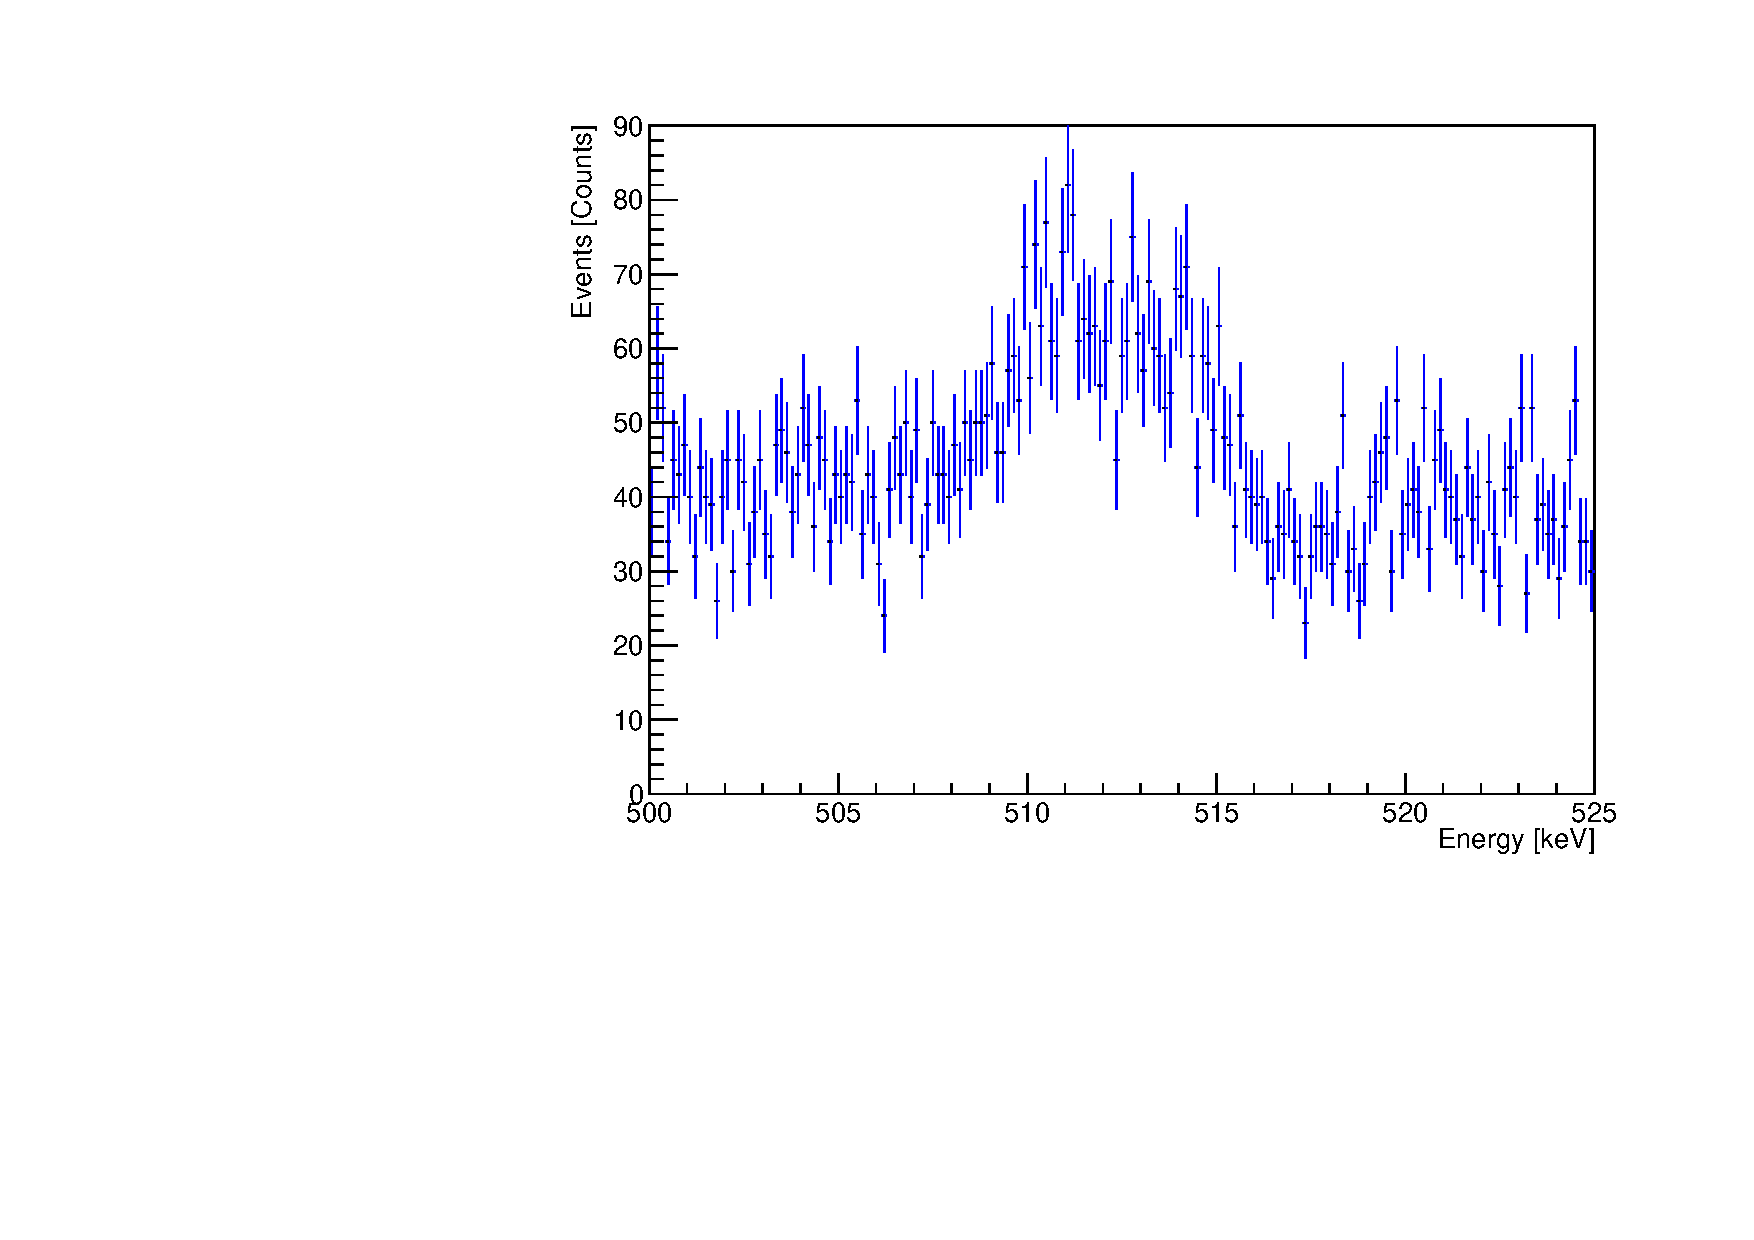
\includegraphics[width=100mm]{./Bilder/GraphNoFiltersAtAllAll.pdf}
	\fi%
	\caption{\label{fig:ungefiltertes500525}
		All events measured by all detectors in the range of 500keV to 525keV with no filter applied showing two overlapping peaks at 511keV and 514keV.
	}
\end{figure}



As it was elaborated in section \ref{sec:ExSetup} all GERDA data is stored in a multi-tier data structure. 
All of the data used in this theses are from either tier 3 or from tier 4.
In these tiers a lot of analysis has already been carried out on the individual events measured. 
Among other things, each event in tier 3 and 4 is given a flag whether or not there was a coincidence of the event with a signal in one of the photomultiplier in the water tank around the liquid argon.
This flag is called the "Muon veto" and it always triggers whenever there is a strong Cherenkov signal measured.
Due to the high energy needed to create any Cherenkov signal no isotope from inside the germanium source and liquid argon and certainly no \nuc{Kr}{85} should trigger the MuiVeto.
This can be used to filter out high-energy particles from outside and the background they create.
\\

For a photon of a rare \nuc{Kr}{85} decay to create the distinct 514keV peak it is necessary that it has to deposit all of its energy in only one of the detectors. 
This means that any energy measured in one Germanium detectors that has a coincidence with a non neglectable signal measured in another Germanium detector is most likely not a real rare \nuc{Kr}{85} decay.
Whether an event has more than one detector measure a signal can be determined by the multiplicity counter of each event stored in tier 3 and 4.
Using this counter even more background of none \nuc{Kr}{85} can be repressed by only using events where only one detector was triggered.
\\

\begin{figure}[t!]
	\centering
	\ifmakefigures%
	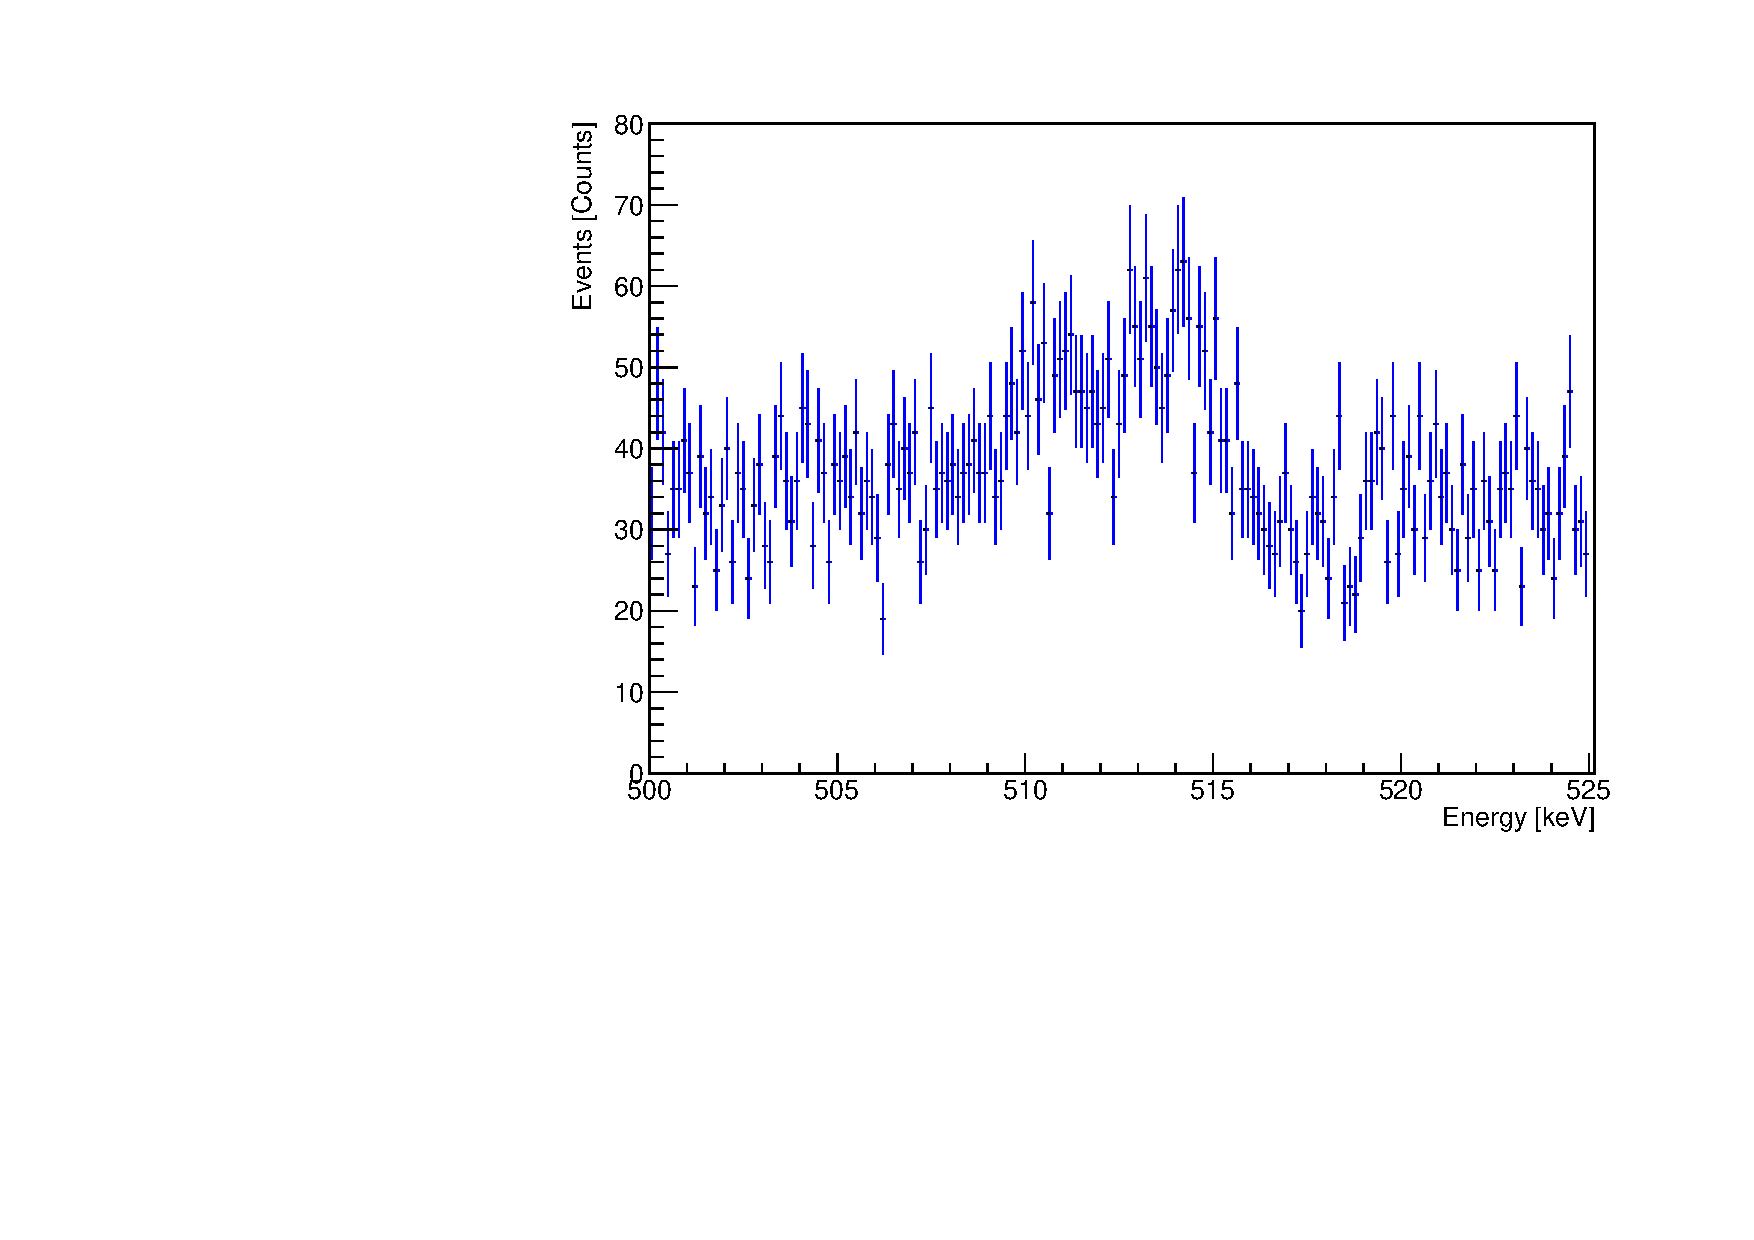
\includegraphics[width=100mm]{./Bilder/500525NoFilterAllDetectors.pdf}
	\fi%
	\caption{\label{fig:leichtGefiltertes500525}
		All events measured by all detectors in the range of 500keV to 525keV with the Mui Veto and only one detector triggered.
	}
\end{figure}

With these two filters you get a new graph with less background seen in figure \ref{fig:leichtGefiltertes500525}.
One can see that the annihilation events could be partially suppressed by these two filters making the two peaks more distinguishable.
From now on, only those events that came through these two filters will be used in further analysis.
\\

After applying the first few rather general filters on the measured events one has to make a distinction between the events measured in different kinds of detectors.
As it was elaborated in section \ref{sec:ExSetup}, two different types of detectors were used in the GERAD experiment - the BEGes (Broad Energy Germanium diods) and the COAX (coaxial diods). 
Due to their differences in design and weigh the two types have a different energy resolution. 
The BEGes are generally smaller and therefor have a higher energy resolution compared to the rather big COAX detectors.
For example, in the range of 500keV it can be expected that COAX have a resolution about 0.5keV higher than the BEGes \cite{2017Natur.544...47A}. 
Because of this their measured data must and will be evaluated separately. 
If you only take the events that are recorded in the respective detectors, you get figure \ref{fig:NoFilterBEGes} for all the events measured in the BEGe detectors and figure \ref{fig:NoFilterCOAX} for all the events in the COAX detectors.
The difference in resolution can be seen in the fact that in the BEGe diagram the two peaks are distinguishable while they merge into one another in the COAX diagram.  
\\

\begin{figure}[t!]
\centering
\begin{minipage}{.5\textwidth}
  \centering
	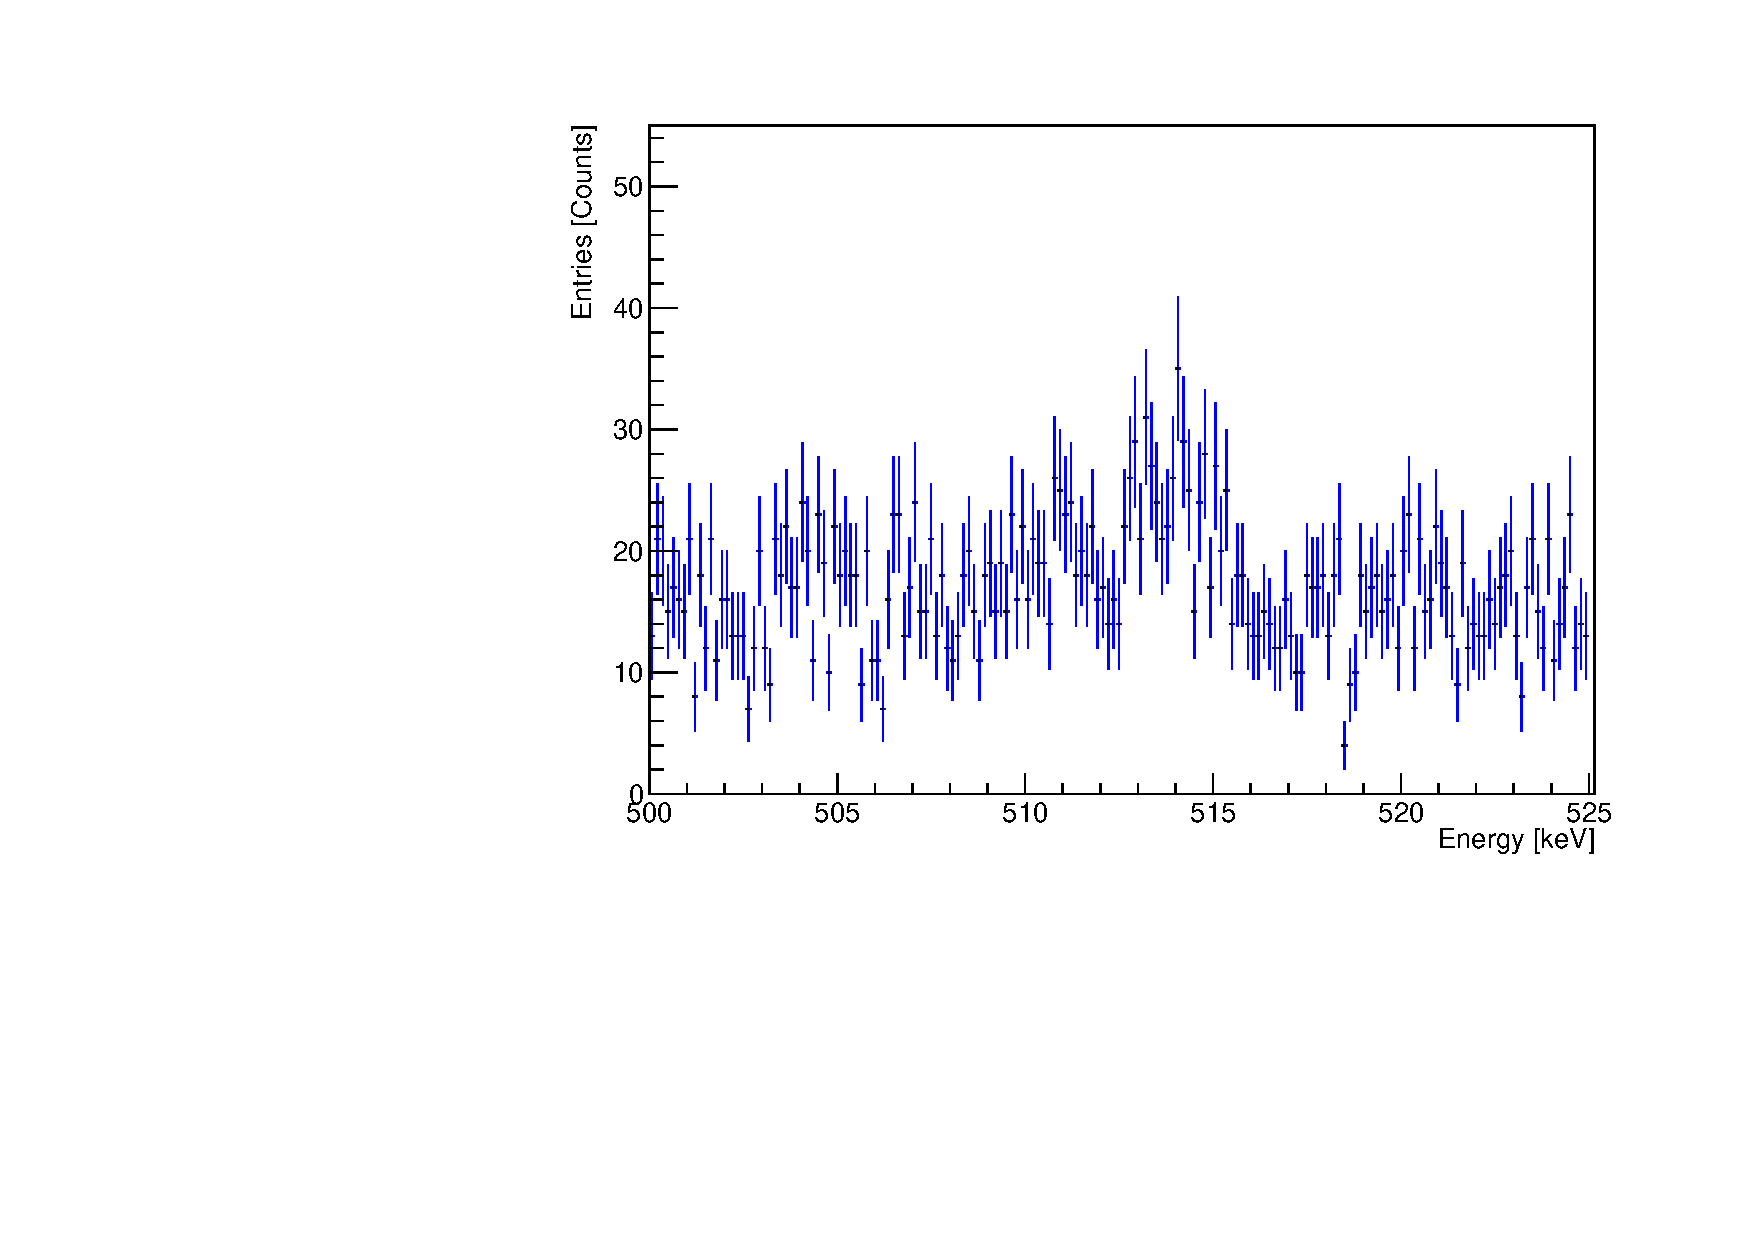
\includegraphics[width=80mm]{./Bilder/500525NoFilterBEGes.pdf}
  \label{fig:NoFilterBEGes}
  \caption{BEGes}
\end{minipage}~
\begin{minipage}{.5\textwidth}
  \centering
	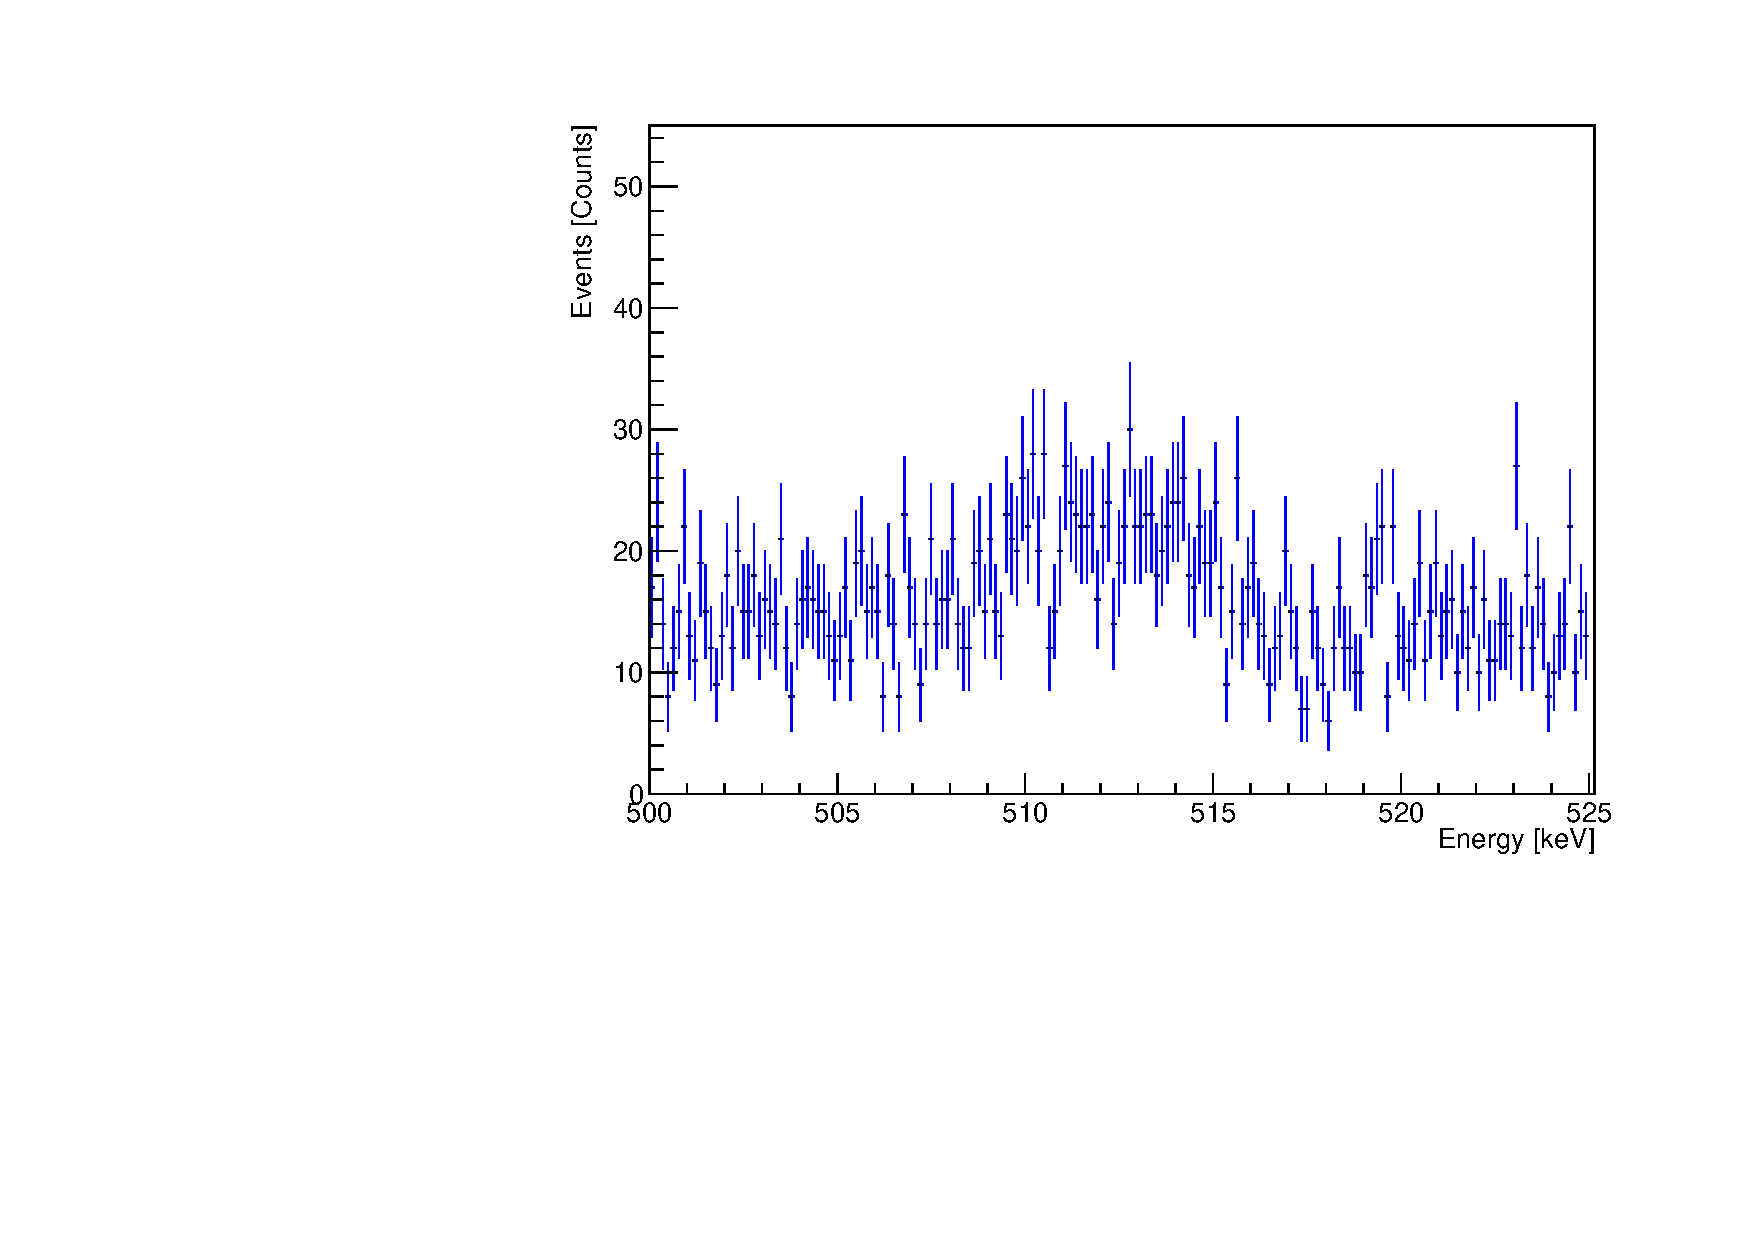
\includegraphics[width=80mm]{./Bilder/500525NoFilterCOAX.pdf}
  \caption{COAX}
  \label{fig:NoFilterCOAX}
\end{minipage}
    \\
	\vspace{0.5cm}
	All events measured by the respective detectors in the range of 500keV to 525keV.
\end{figure}

At this point it is clear that we have two options on how we can handle the problem of the positron electron annihilation peak. 
Either we try to find a way to filter out the majority of the annihilation events while keeping almost all of the \nuc{Kr}{85} events.
This can hopefully be done by using the liquid argon veto of GERDA and the precoincidence of the electron scintillation in the photomultipliers. 
\\
The other option is to leave the phase-space diagram as it is and we only change our fit function so that it also takes the second peak into account when fitting.
But this is only really an option for the BEGe detectors.
As mentioned earlier the peaks in the BEGe phase-space are clearly distinguishable while they merge into each other in the COAX diagram.
This merging of the peaks makes it difficult to put a clear fit function through the two peaks.
Also considering the fact, that the COAX detectors have a corser resolution than the BEGe detectors, in the further analysis only the values of the BEGe detectors will be used.
Nevertheless, the results of the COAX detectors can give us a reinsurance that the value is at least in the right order of magnitude.
\\

In this theses we will try to go both ways separately and later compare their informative value.
But first we need to discuss how we want to suppress the annihilation peak and whether our method really makes sense. 
This will be done in the following chapter.
\\


\subsubsection{Annihilation peak suppression}
\label{sec:APS}

As mentioned above, it should be theoretically possible to filter out the majority of the disturbing positron electron annihilation events by using the scintillation property of the liquid argon.
In the case of the rare \nuc{Kr}{85} decay the emitted electron has a very low mean kinetic energy of E\(_{mean}=47.65\)keV.
This means that in the majority of these rare decays no light should be seen in the detectors because the beta electron is unlikely to trigger any of them.
In contrast to that you can expect a very strong light signal every time a positron electron annihilation occurs. 
One should therefor be able to filter out almost all of the annihilation events while keeping the majority of the \nuc{Kr}{85} decay by only using events where this flag is not triggered.
This chapter tries to implement a filter that uses this mechanism and discusses in the end how successful the repression really was.
\\

Among other things, each event in tier 4 was given a flag called "isLArVetoed".
This flag is always triggered whenever an event in the Germanium detectors coincides with a strong scintillation signal in one of the photomultipliers positioned in the liquid argon tank.
In particular, the signals in the photomultipliers must have an intensity of at least 0.5 phe for them to trigger the flag \cite{2017Natur.544...47A}.
If one plots all events in which this flag has not been set one gets figure \ref{fig:LArBEGes} for the BEGes and figure \ref{fig:LArCOAX} for the COAX detectors.
You can see that the positron electron annihilation peak can not be identified any longer while the 514keV peak seems almost unchanged.
\\

\begin{figure}[t!]
\centering
\begin{minipage}{.5\textwidth}
  \centering
	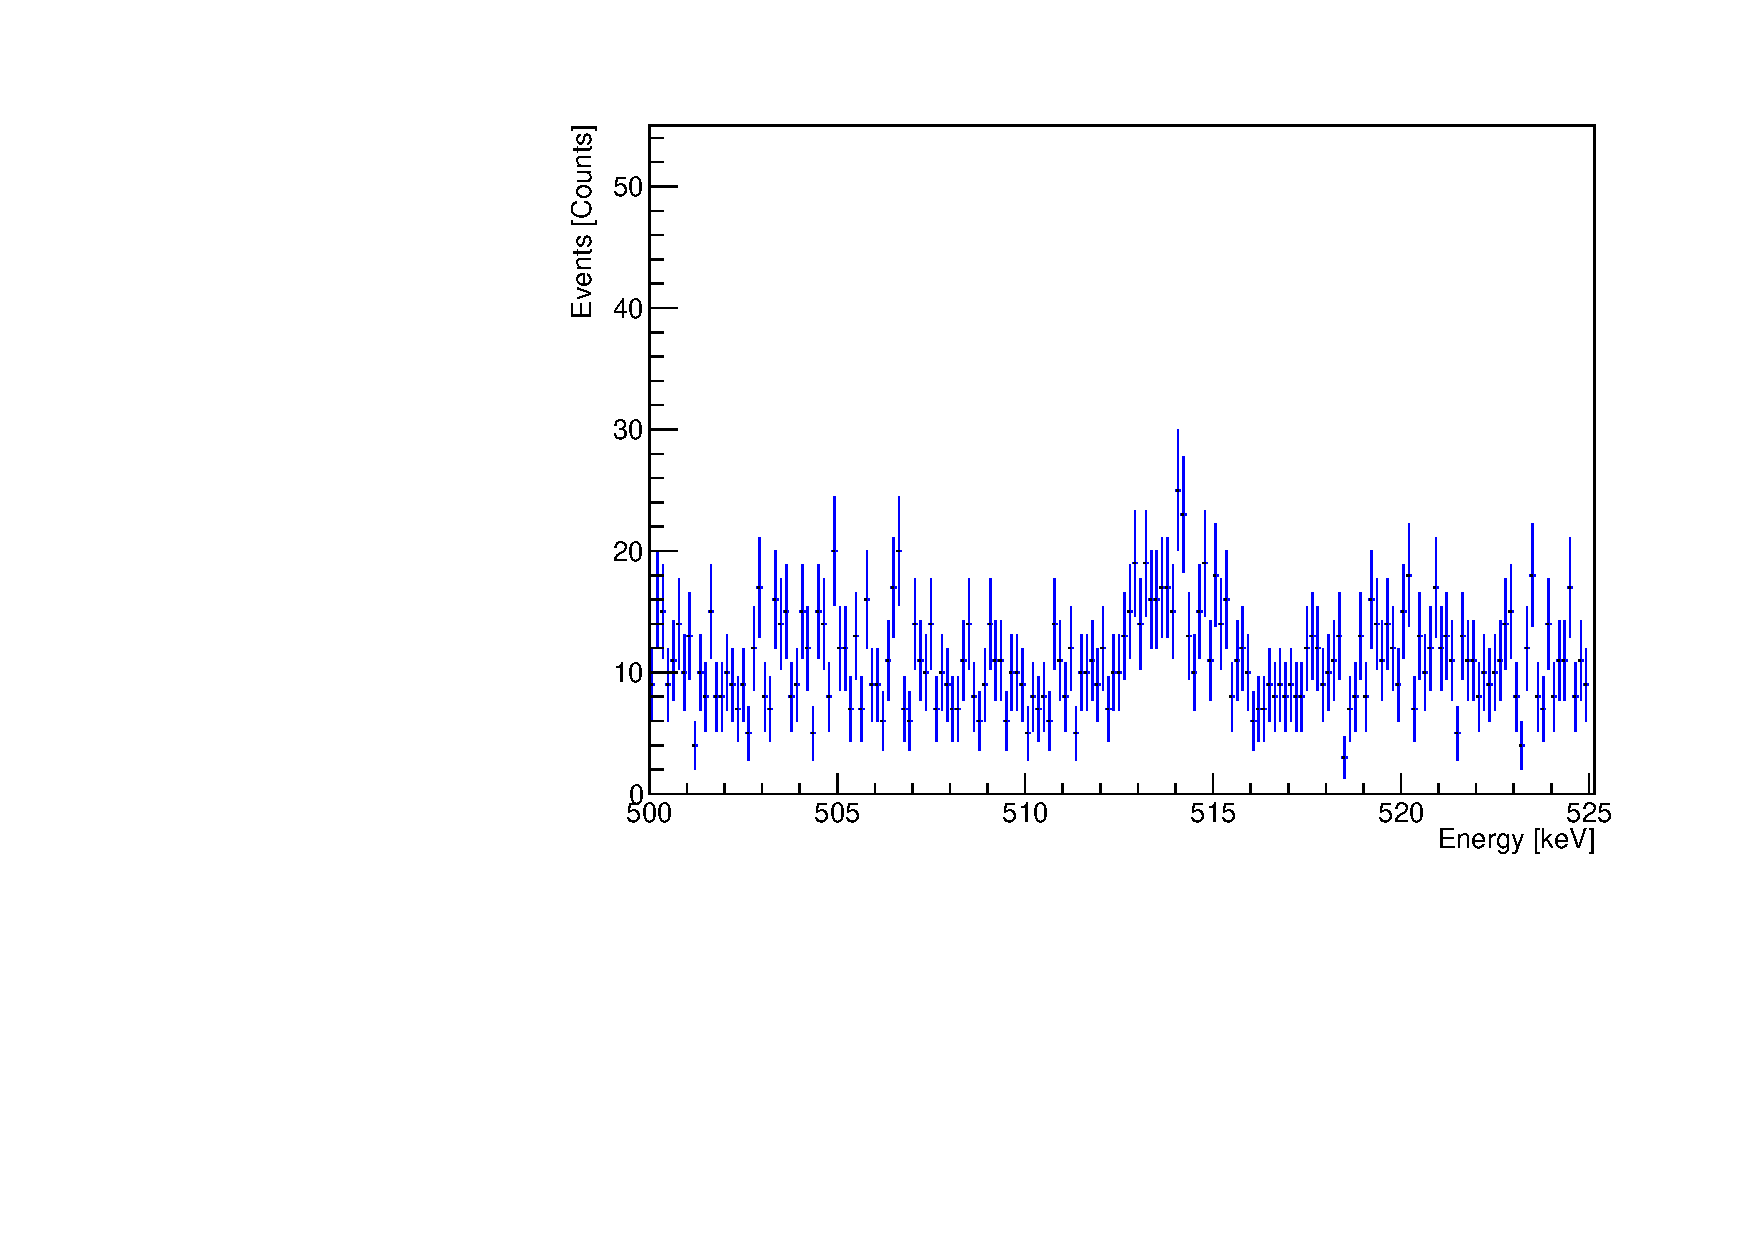
\includegraphics[width=80mm]{./Bilder/500525LArVetoBEGes.pdf}
    \caption{BEGes}
  \label{fig:LArBEGes}
\end{minipage}%
\begin{minipage}{.5\textwidth}
  \centering
	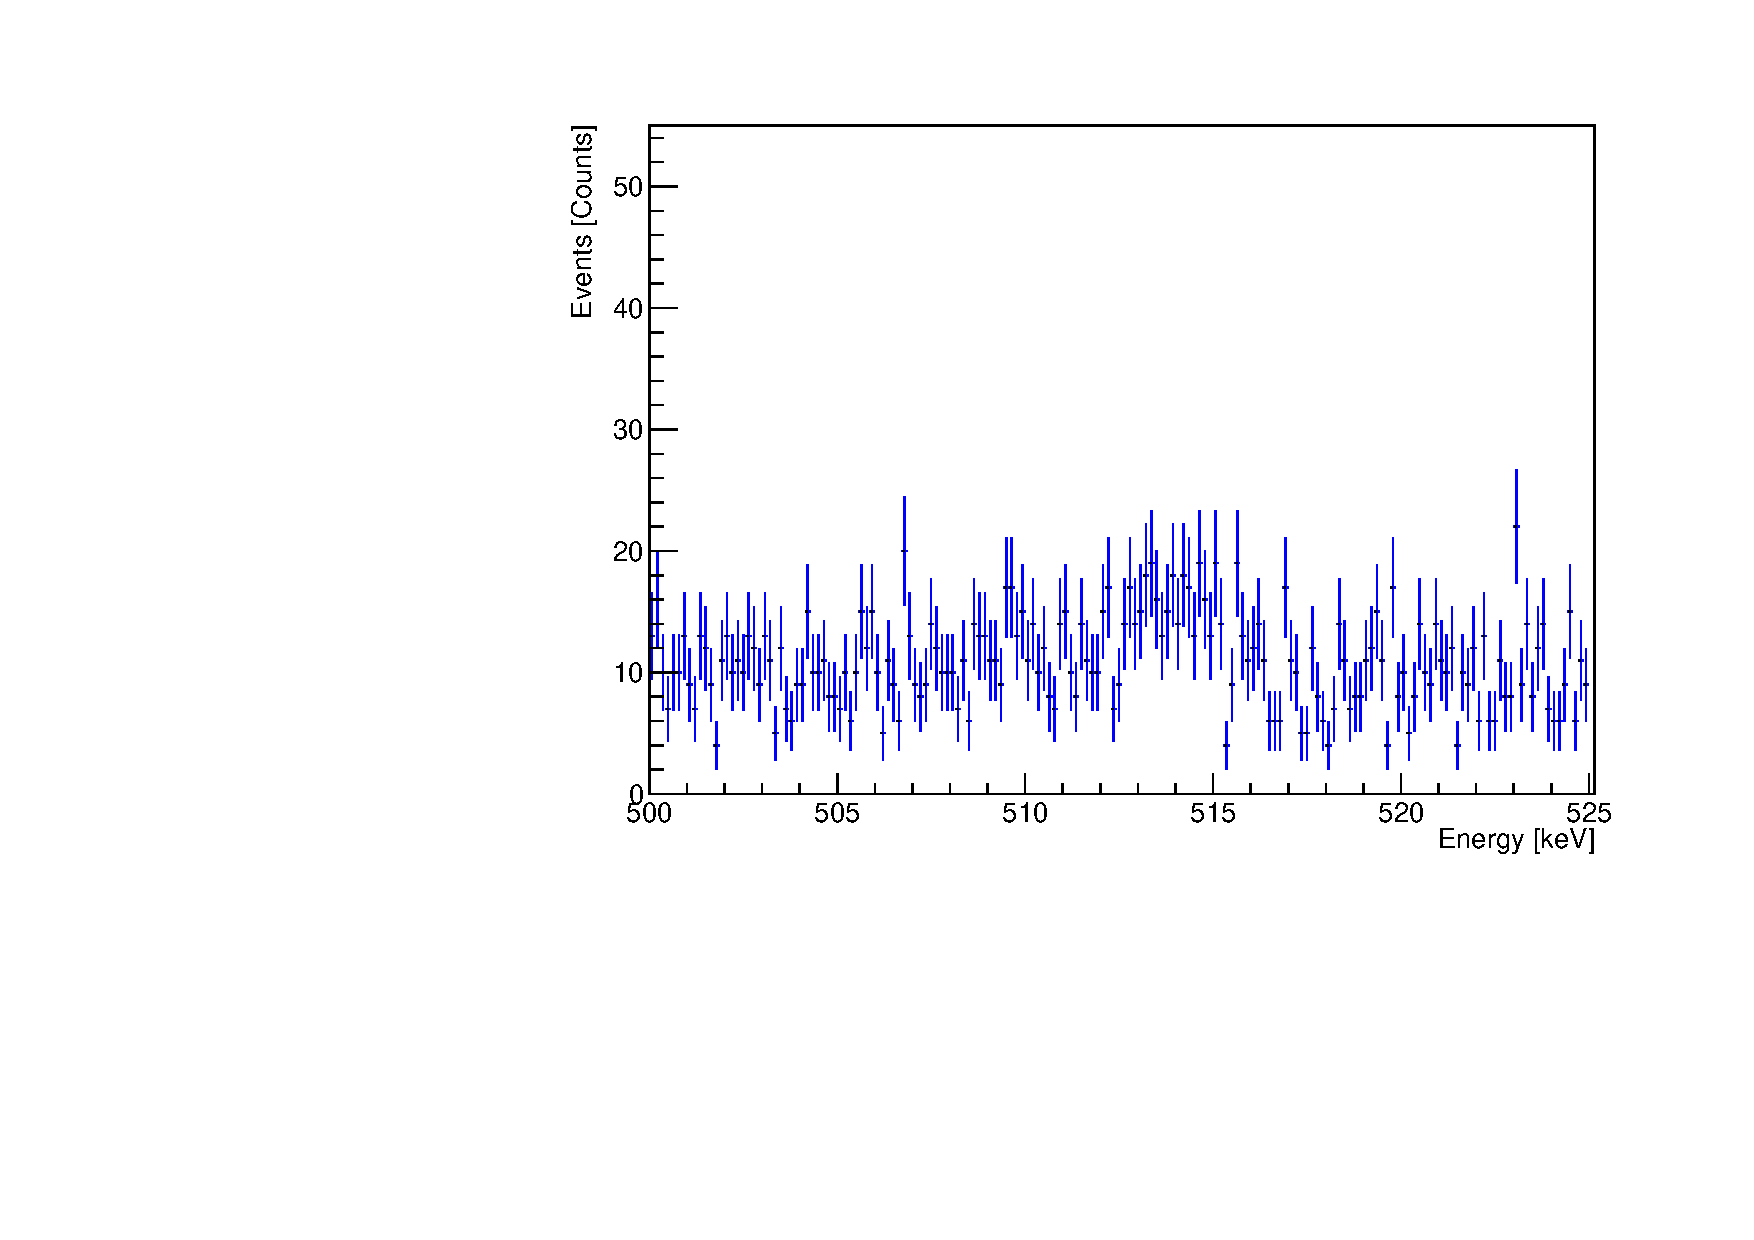
\includegraphics[width=80mm]{./Bilder/500525LArVetoCOAX.pdf}
  \caption{COAX}
  \label{fig:LArCOAX}
\end{minipage}
    \\
	\vspace{0.5cm}
    All events measured by the respective detectors with the LAr filter applied in the range of 500keV to 525keV.
\end{figure}

At this point one could say that we have done enough filtering and use this graph to determine the number of decays in the peak.
But due to the non vanishing possibility of the beta electron to trigger the liquid argon veto it is of interest to investigate whether the filter has accidentally filtered out any real rare \nuc{Kr}{85} decay and whether it is possible to recover them.
The number of events filtered out by the liquid argon veto in the energy range of 509 to 519 keV is 1728.
This number is way too big to look at every individual case.
\\

Luckily we can use the fact that the excited \nuc{Rb}{85} state has a half life of 1.015 \(\mathrm{\mu}\)s.
This means that we can identify potential real rare \nuc{Kr}{85} decay by looking exclusively at the events in which the trigger from the photomultiplie happened earlier then the Germanium detector event.
In other words, we only use events with a negative time difference between these two events.
The time difference for each individual liquid argon events is already analyzed and stored in the triggerLAr vector of the Tier 3 dataset.
This vector has the same number of dimensions as there are photomultipliers and every entry is indexed with the corresponding input channel of this photomultiplier.
The entries of this vector are again vectors themselves storing the time difference for every signal that triggered the liquid argon veto in the corresponding channel.
Since the events are listed in ascending order and we are interested in the first trigger event of the photomultiplier, we use only the first entry of this inner vector here for simplicity.
\\

In addition, we also know that the energy of the released beta electron is relatively low.
This means that we can expect that only a small number of photomultipliers should measure a signal in a real rare \nuc{Kr}{85} decay.
In this case we will only use those events that have a maximum of four different triggered photomultipliers.
Allowing events with maximum of four different triggered photomultipliers is already a lot for a \nuc{Kr}{85} decay. 
But we wanted to do a more detailed manually investigation later anyways which is why the filter can be a little coarser here.
\\

\begin{figure}[t!]
	\centering
	\ifmakefigures%
	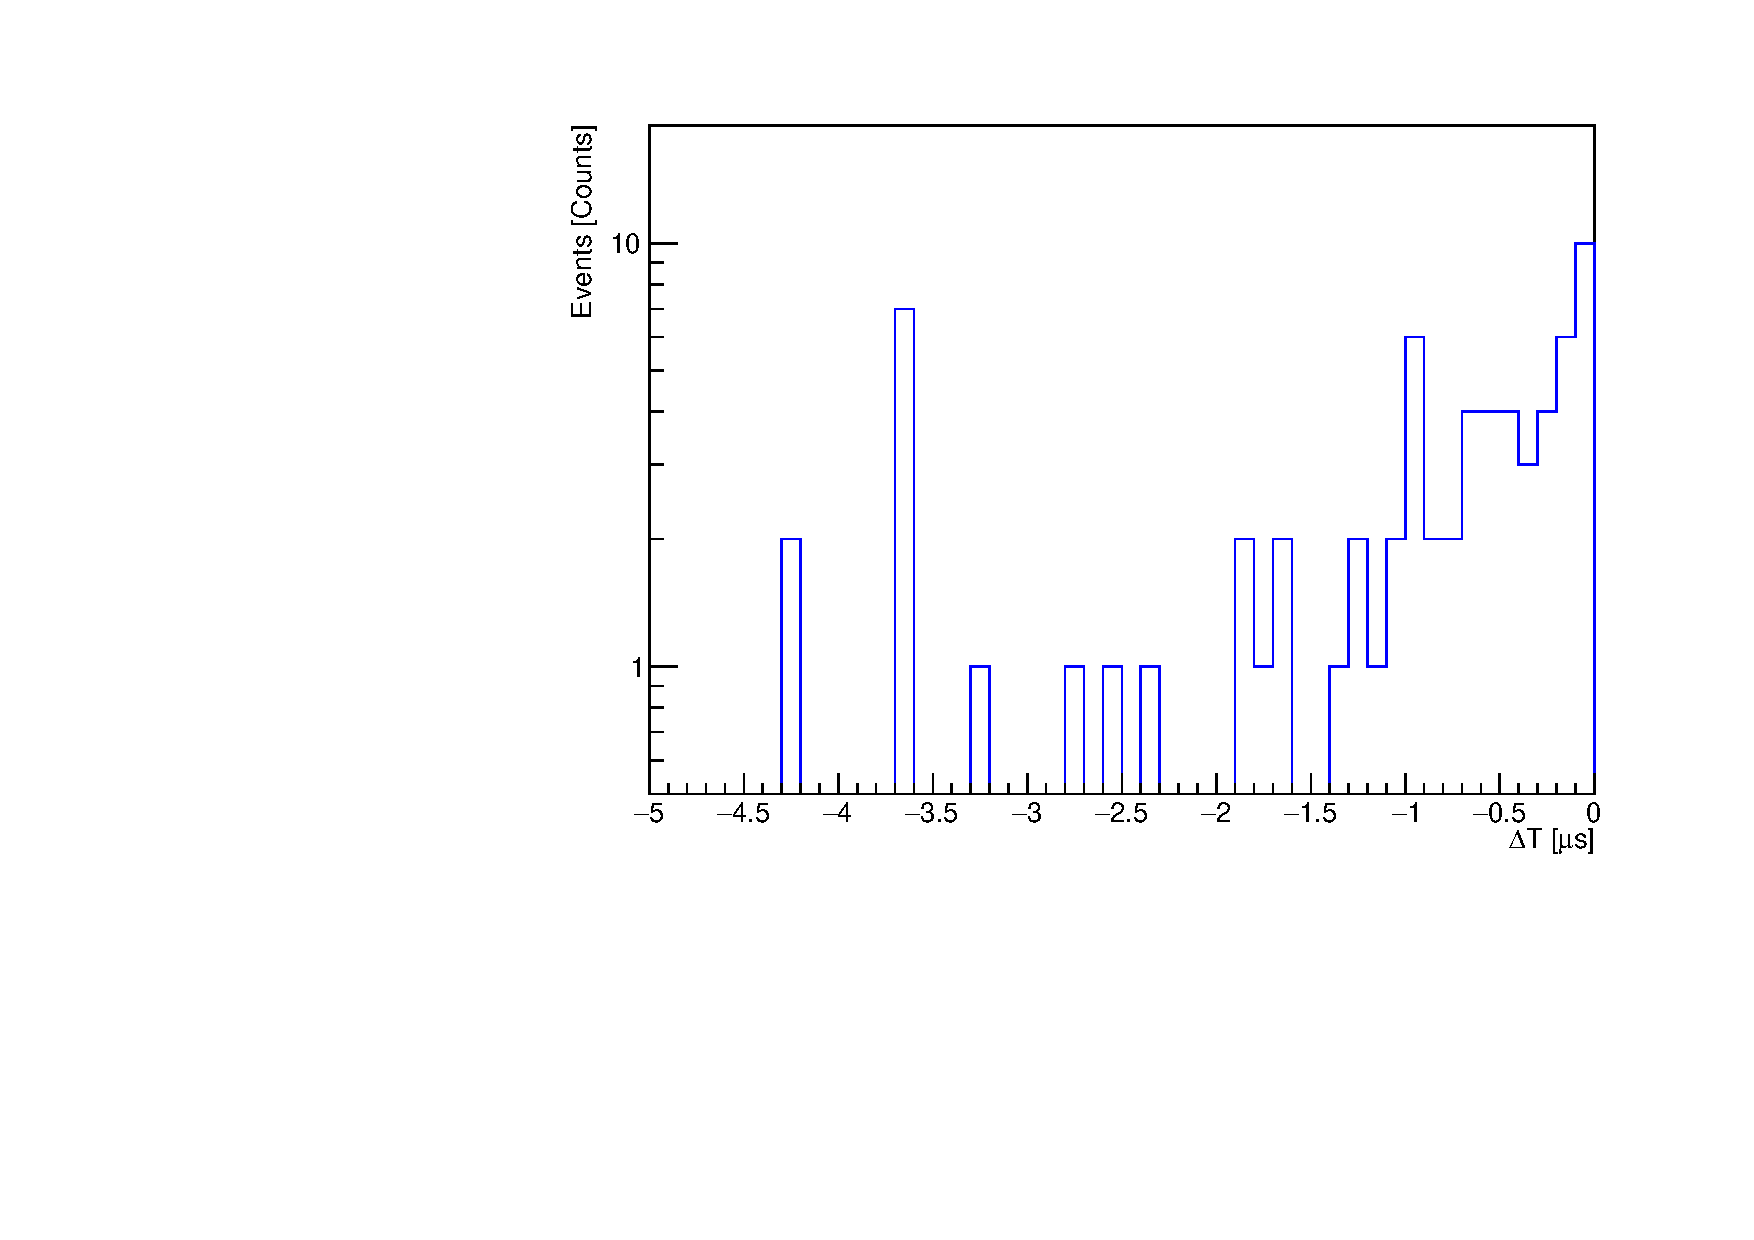
\includegraphics[width=100mm]{./Bilder/TriggerTimeOnly4.pdf}
	\fi%
	\label{fig:Trigger4}
	\caption{
		All liquid argon filtered events with a negative time difference between the event in the Germanium detector and a signal in the photomultipliers in the liquid argon tank.
	}
\end{figure}

If you apply these two restrictions to the liquid argon filtered events and only take those photomuliplier signals with a signal strength of at least 0.5 phe you get a distributions as seen in figure \ref{fig:Trigger4}.
We are only interested in the signals that measured at least 0.5 phe because, as mentioned above, that is the necessary intensity to trigger the LAr veto making them the signals of interest. 
The x axis is the time difference of the events in the photomultipliers from the signal measured in one of the Germanium detectors.
Theoretically it should now be possible to see a exponential increase from the negative scale towards a vanishing time difference.
Because of the small number of events however, it is almost impossible to make any statements about the course of these events.
\\

Interestingly, the majority of all signals were measured with a negative time difference in the PMTs. 
This could perhaps be due to the better temporal resolution of the PMTs. 
The signals of all PMTs are recorded with a resolution of 10ns and the SiPM with a resolution of 80ns but over a larger range than the PMTs\cite{nature}. 
However, since the expected time difference is in the order of \(\mu\)s, this is no reason for the reduced number of measured events. 
Another difference between the photomultiplier types is that the PMTs have a faster reaction time than the SiPMs. 
As we will see, practically all deflections in the measured intensity of the PMT signal caused by procoincedents have already subsided before the signal was measured in the germanium detectors. 
Thus a clear maximum should be recognizable before the germanium detector events.
In contrast, the measured signal of the SiPMs increases exponentially with a characteristic time in the order of 10\(\mu\)s. 
The trigger positions are then determined by software. 
However, this should still be able to determine the trigger position of the signals for procoincedence events with sufficient accuracy.
!!!!! Hier dir noch was genaueres ausdenken !!!!!
\\

Nevertheless we were able to lower the number of potential \nuc{Kr}{85} events from 1728 down to only 55.  
These remaining events can now be manually examined with a with software called GerLa written by GERDA employees.
This tool allows one to search for a specific event and see all recorded signals of the Germanium detectors and the photomultipliers around this event.
\\

With this program one can now perform a manual filter by looking at the remaining 55 events indivitually and perform a specific protocol to determin wheter they are signals from a rare \nuc{Kr}{85} decay or not.
This protocol consists of filtering out every event that has a combined light intensity of over 4 phe, every event that only has a negative time difference in a signal weaker than 0.5 phe and every event in which a pileup distorted the signal.
Due to their higher sensitivity, the signal of the photomultiplier tubes (PMT) was mainly but not exclusively used.
The silicon photomultipliers (SiPM) have the downside of a slower reaction time and the majority of events in them that happened before the Germanium signal were background events.
In figure \ref{fig:Beispiel1} is an example for a model signal in the PMT.
\\

\begin{figure}[t!]
	\centering
	\ifmakefigures%
	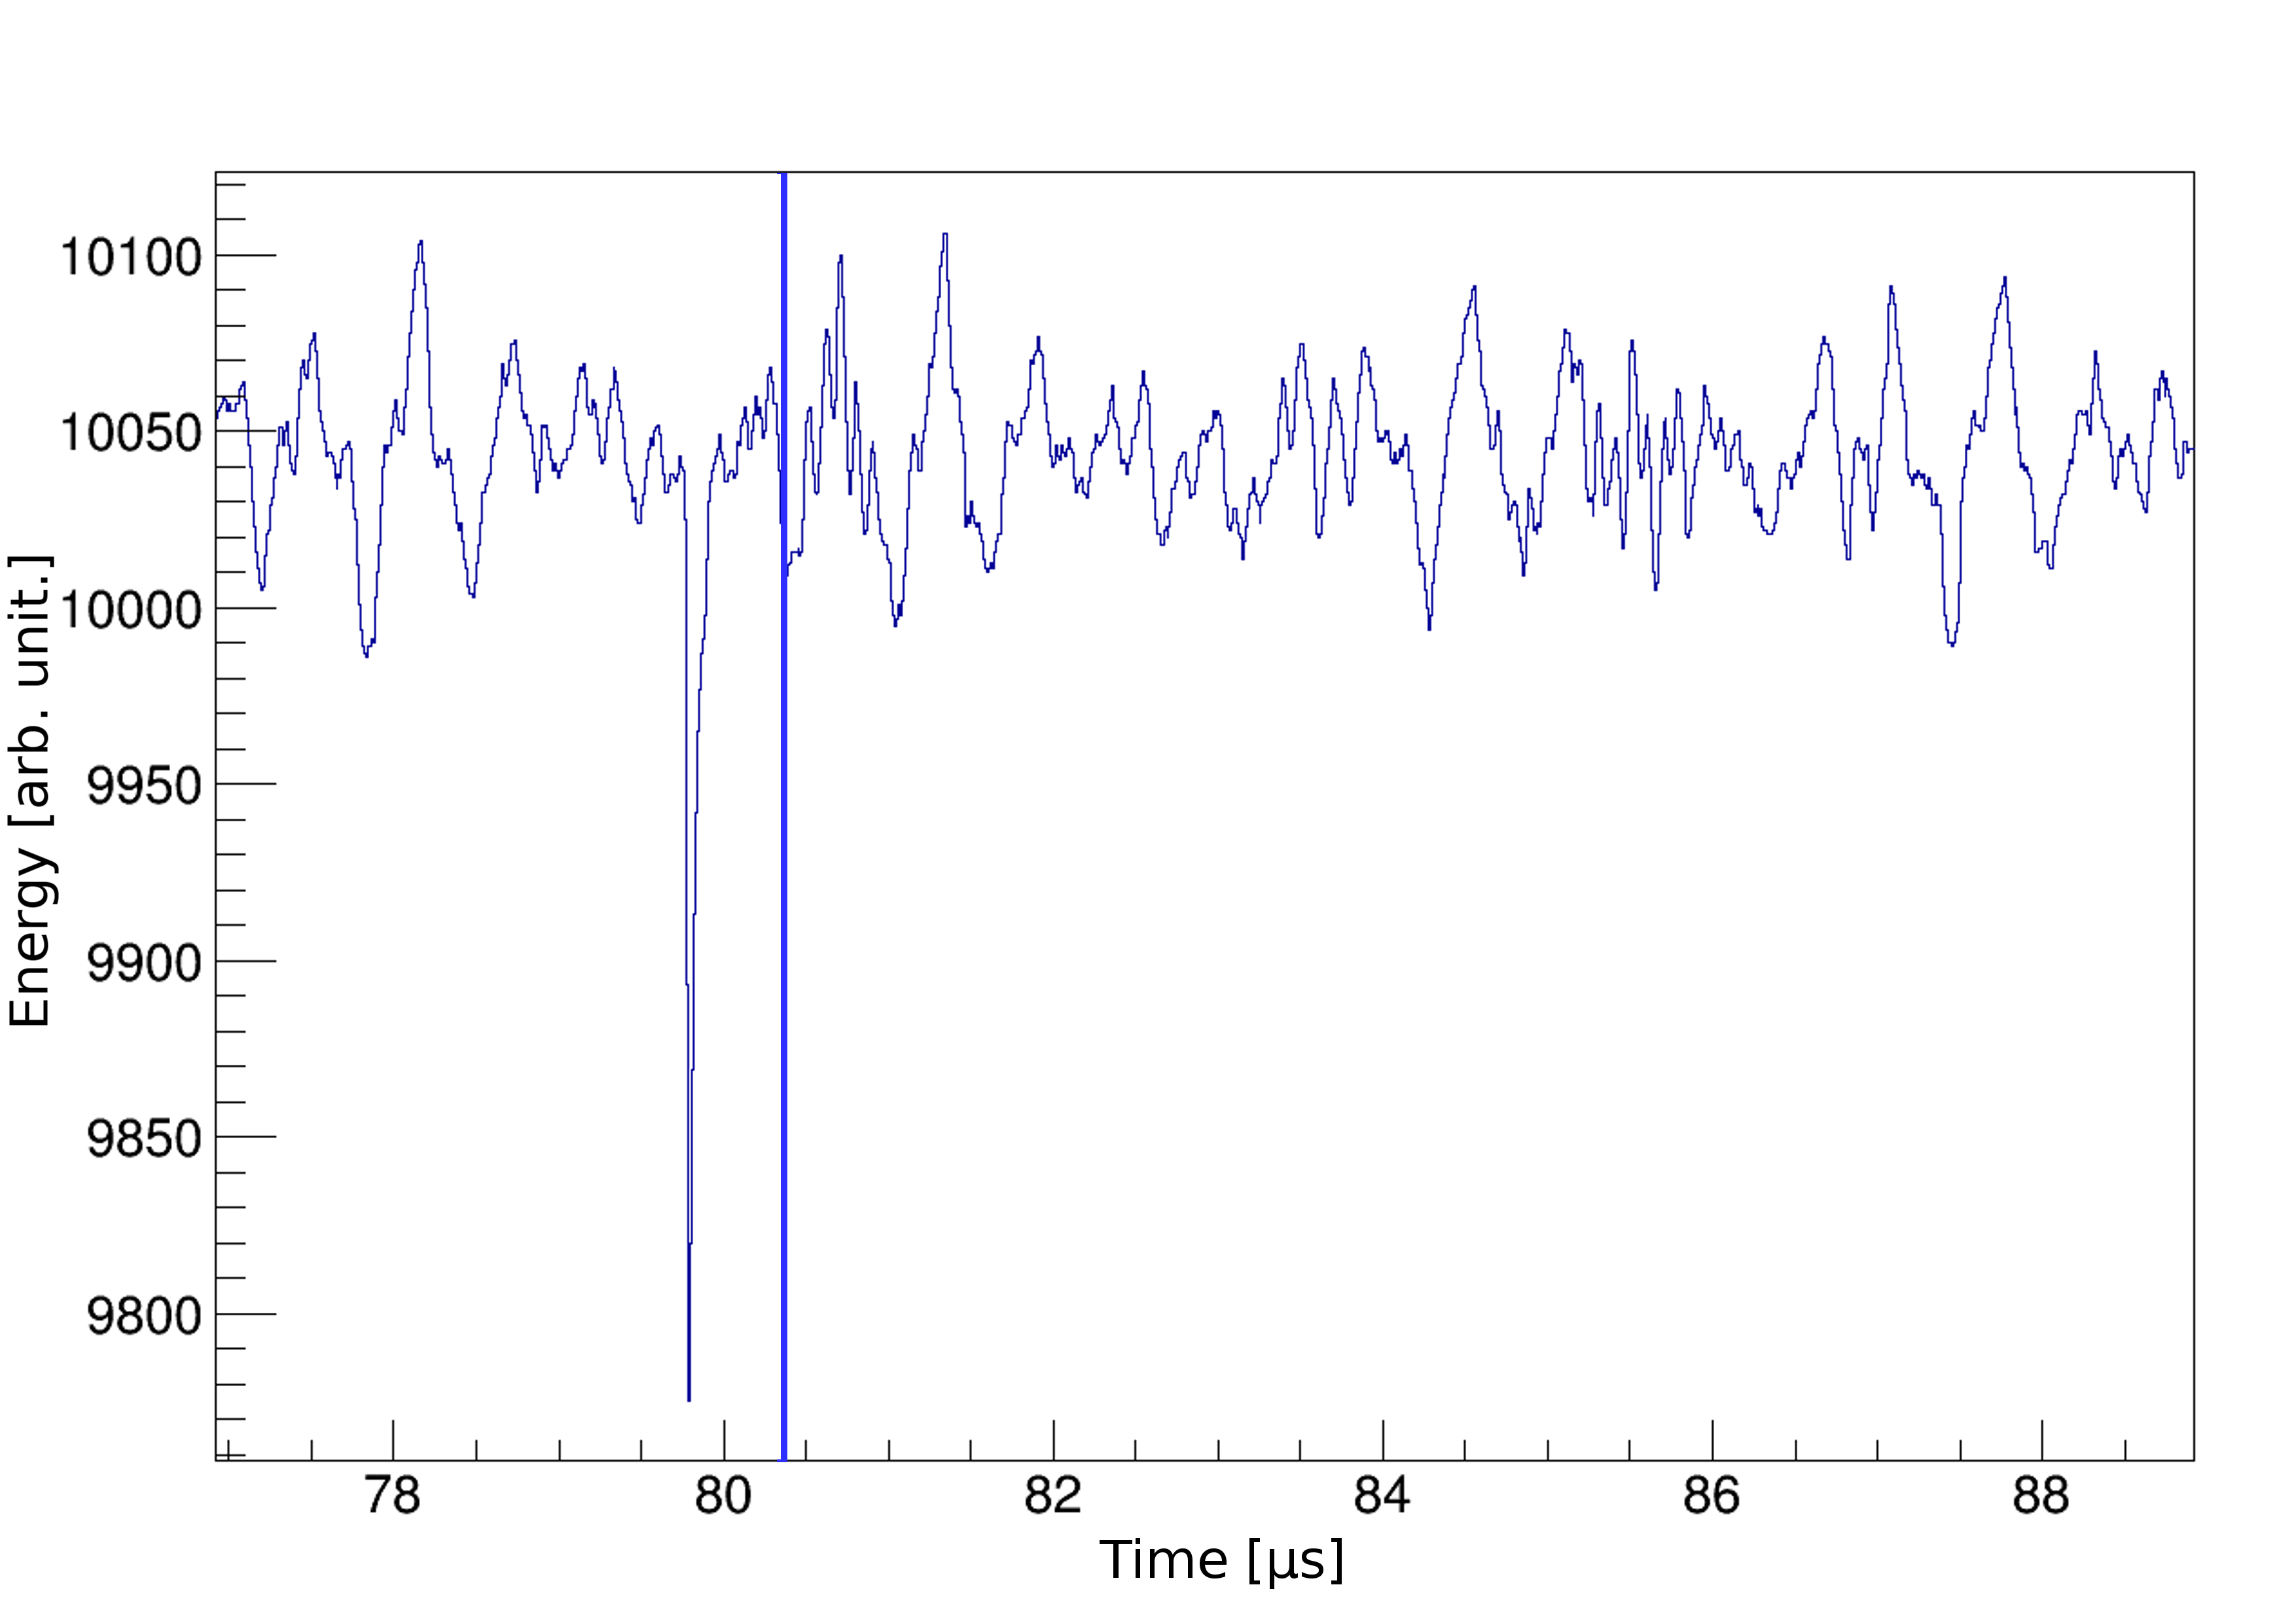
\includegraphics[width=100mm]{./Bilder/BeispielSignal.png}
	\fi%
	\caption{\label{fig:Trigger4}
    The recorded signal of the photomultiplier tube P4 from the event with event number 1614036. !!!!!Hier noch was zu den Achsen!!!!!. 
    The blue bar represents the moment in time in which a signal in the Germanium detector was measured.
	}
\end{figure}

Using this procedure we were able to lower the amount of possible rare \nuc{Kr}{85} decay signals down to 24 events.
After this much filtering we can assume that all of these events are probably real rare \nuc{Kr}{85} decays.
Finally we can recover those events to our liquid argon filtered energy diagrams (see figure \ref{fig:LArBEGesEV} and \ref{fig:LArCOAXEV}).
You can see in comparison to figure \ref{fig:LArBEGes} and \ref{fig:LArCOAX} that the majority of the recovered events are placed near the 514keV peak.
\\

Now the question arises whether our approach could actually restore the majority of all lost \nuc{Kr}{85} events.
A quantitative statement can only be obtained after a fit function analysis of the graphs to determine amount of actual rare \nuc{Kr}{85} events measured.
This can be done by integrating over the fit function as it will be done in section \ref{sec:Fitting}.
\\

Nevertheless we are still able to make some qualitative estimations about the recovery rate of this approach. 
When trying to make a more realistic estimation one can see qualitatively that the actual portion of recovered events must not be much smaller.
An important factor limiting this recovery rate originates from an approximation applied in this approach.
It was approximated that the electrons created scintillation light instantaneously after being released.
In reality, the moment an electron emits scintillation light is determined by many complex mechanisms. 
However, its behaviour can be approximated by a relaxation approach. 
This gives you a new characteristic time with which you can describe how many electrons have already created scintillation light after what time. 
But this not spontaneous behavior means, that the measured signal depends on both the relaxation time of \nuc{Rb}{85} and the scintillation light of the electron.
It is therefor quite possible, that a number of rare \nuc{Kr}{85} decay events can have a positive effective time difference.
Those are then lost in our analysis due to us filtering out every event that has a positive time difference.
This results in a lower recovery rate.
\\

After this qualitative analysis it is justified to question whether the majority of the rare \nuc{Kr}{85} decays can even pass through the LAr filter and the additional recovery.
But we only get a satisfactory answer with a quantitative analysis which will be performed in the following chapter.
\\

\begin{figure}[t!]
\centering
\begin{minipage}{.5\textwidth}
  \centering
	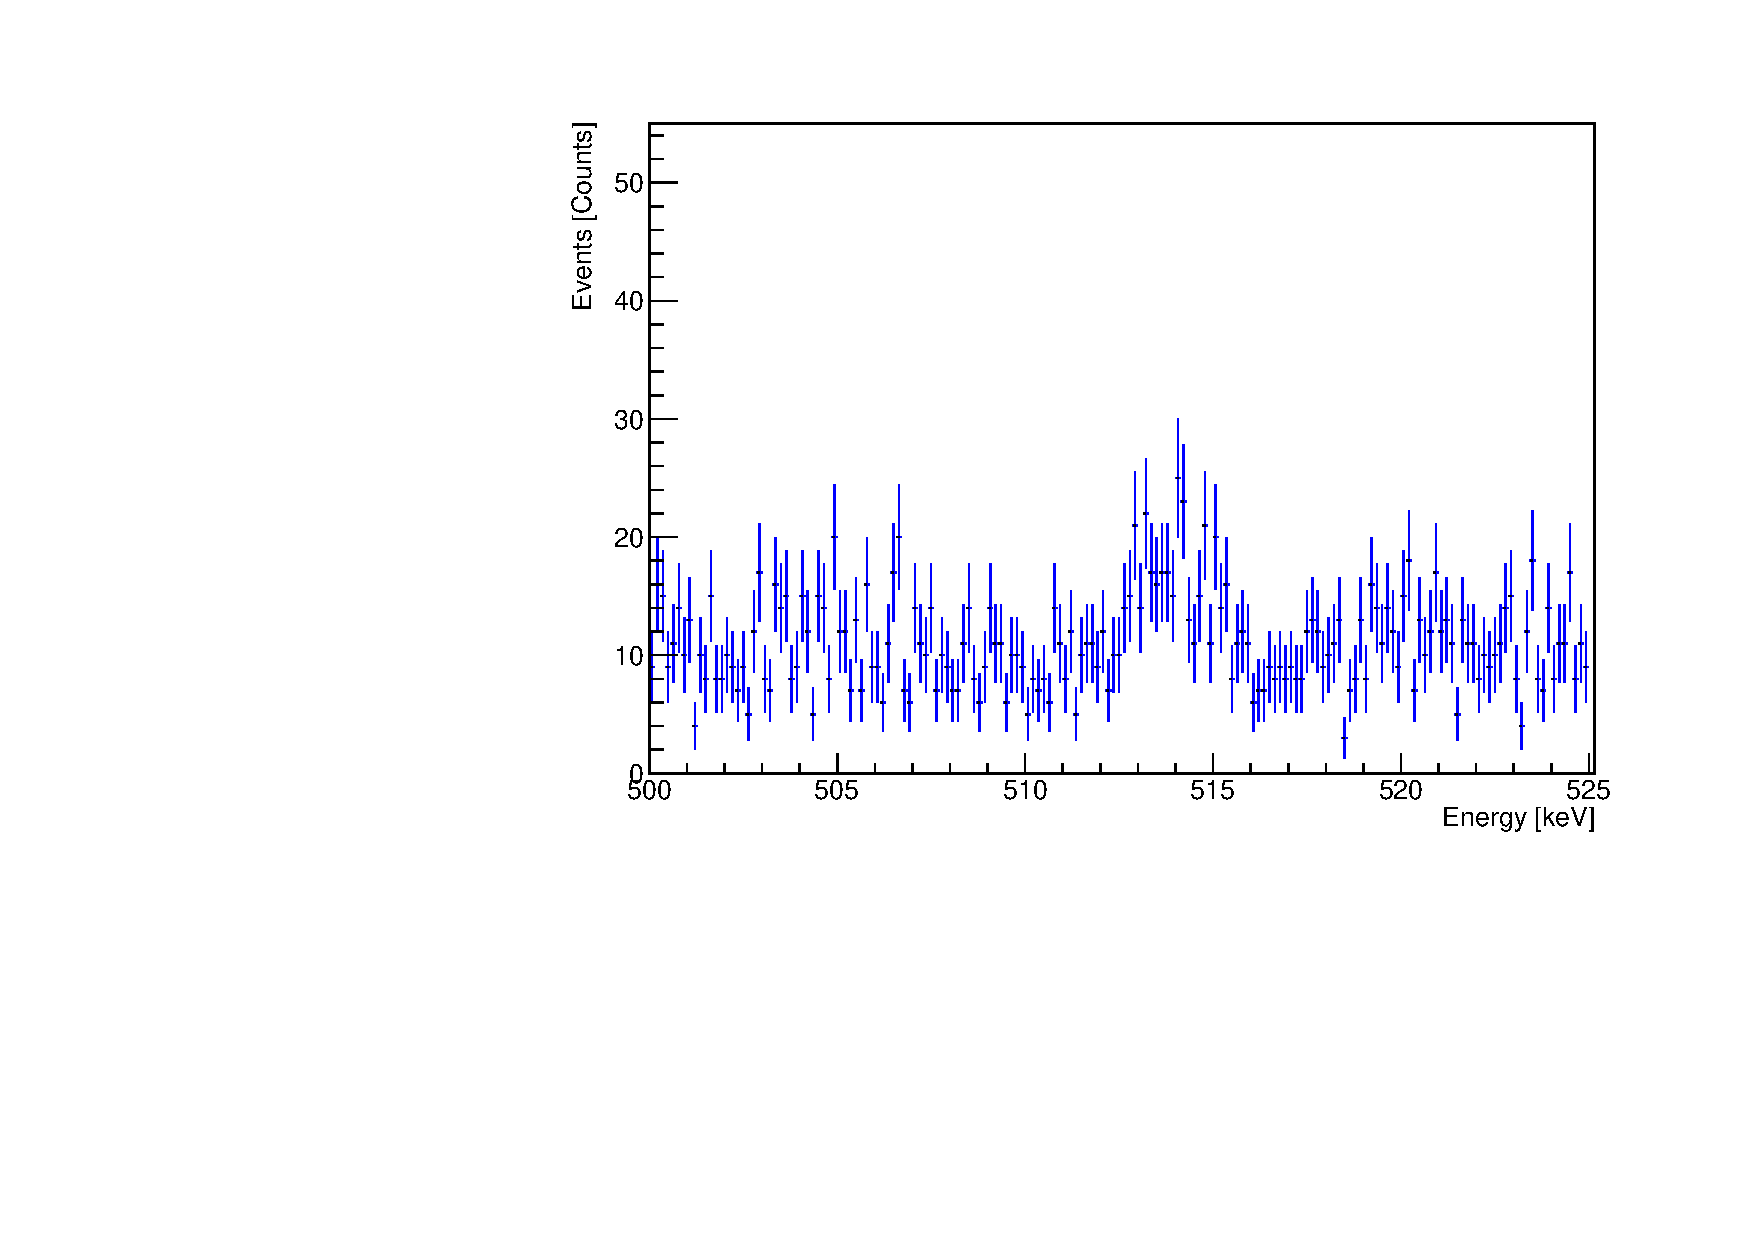
\includegraphics[width=80mm]{./Bilder/500525LArVetoBEGesEventList.pdf}
    \caption{BEGes}
  \label{fig:LArBEGesEV}
\end{minipage}%
\begin{minipage}{.5\textwidth}
  \centering
	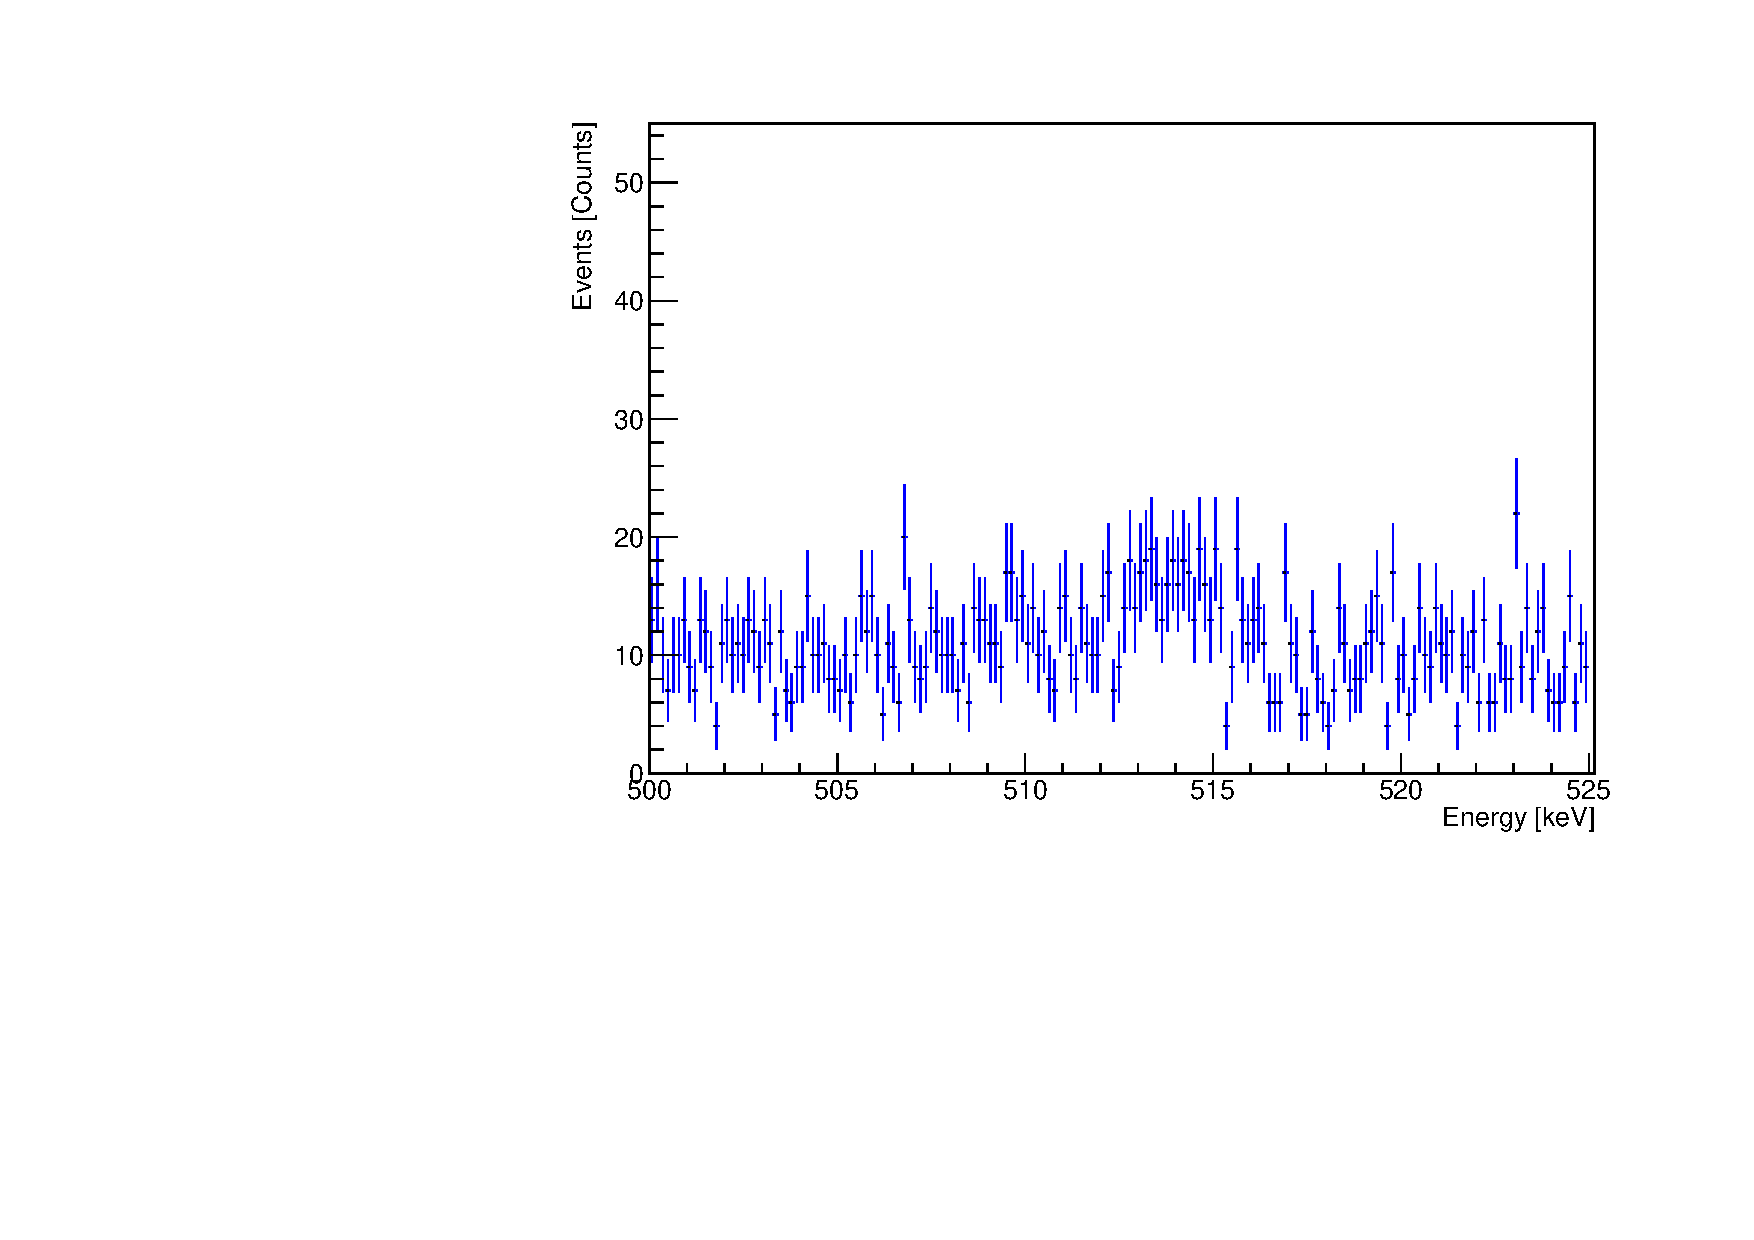
\includegraphics[width=80mm]{./Bilder/500525LArVetoCOAXEventList.pdf}
  \caption{COAX}
  \label{fig:LArCOAXEV}
\end{minipage}
    \\
	\vspace{0.5cm}
    All events measured by the respective detectors with the LAr filter applied and the manually recovered precoincedence events in the range of 500keV to 525keV.
\end{figure}

\subsubsection{Fitting}
\label{sec:Fitting}

Our strategy to calculate the activity of \nuc{Kr}{85} through the 514keV peak involves determining the absolte amount of measured rare \nuc{Kr}{85} decays over all of phase II.
Due to the still enormous amount of events from other sources that can not be suppressed, for example the \nuc{Ge}{67} decays, it is necessary to fit the 514keV peak with a suitable fit function.
The amount of measured rare \nuc{Kr}{85} decays can then be calculated by integrating over the found fit function.
\\

The less filtered phase diagrams \ref{fig:NoFilterBEGes} and \ref{fig:NoFilterCOAX} show two peaks.
This requires the fit function to include two Gaussian functions from which only the parameters of the rare \nuc{Kr}{85} decay will then be analyzed.
Additionally to the two Gaussian peaks a constant and an exponential background function will be added.
Theoretically you can expect the distribution of the germanium events behaves like its phase-space function and should therefor not be constant.
In this case however is the inspected energy interval small compared to the complete phase-space diagram of \nuc{Ge}{67}.
This allows the approximation of the background to change like an exponential function due to the also very little changing background in this interval.
The resulting fit function is shown in equation \ref{equ:FitNoFilters}.
\\

\begin{equation}
\mathrm{f}(x) = \mathrm{A}\frac{1}{\sqrt{2\pi\mathrm{C}}}\exp\left(-\frac{(x-\mathrm{B})^2}{2\mathrm{C}^2}\right) + \mathrm{D}\frac{1}{\sqrt{2\pi\mathrm{F}}}\exp\left(-\frac{(x-\mathrm{E})^2}{2\mathrm{F}^2}\right) + \mathrm{G}\exp\left(\mathrm{H}x\right) + \mathrm{I}
\label{equ:FitNoFilters}
\end{equation}
\\

When you apply the fit function to the two different phase-space diagrams of the two kinds of detectors you get the graphs displayed in figure \ref{fig:FitNoFilterBEGes} and \ref{fig:FitNoFilterCOAX}.
The resulting fit parameters are listed in table \ref{tab:FitParNoFilter}. 
\\


\begin{figure}[t!]
	\centering
	\begin{minipage}{.5\textwidth}
		\centering
		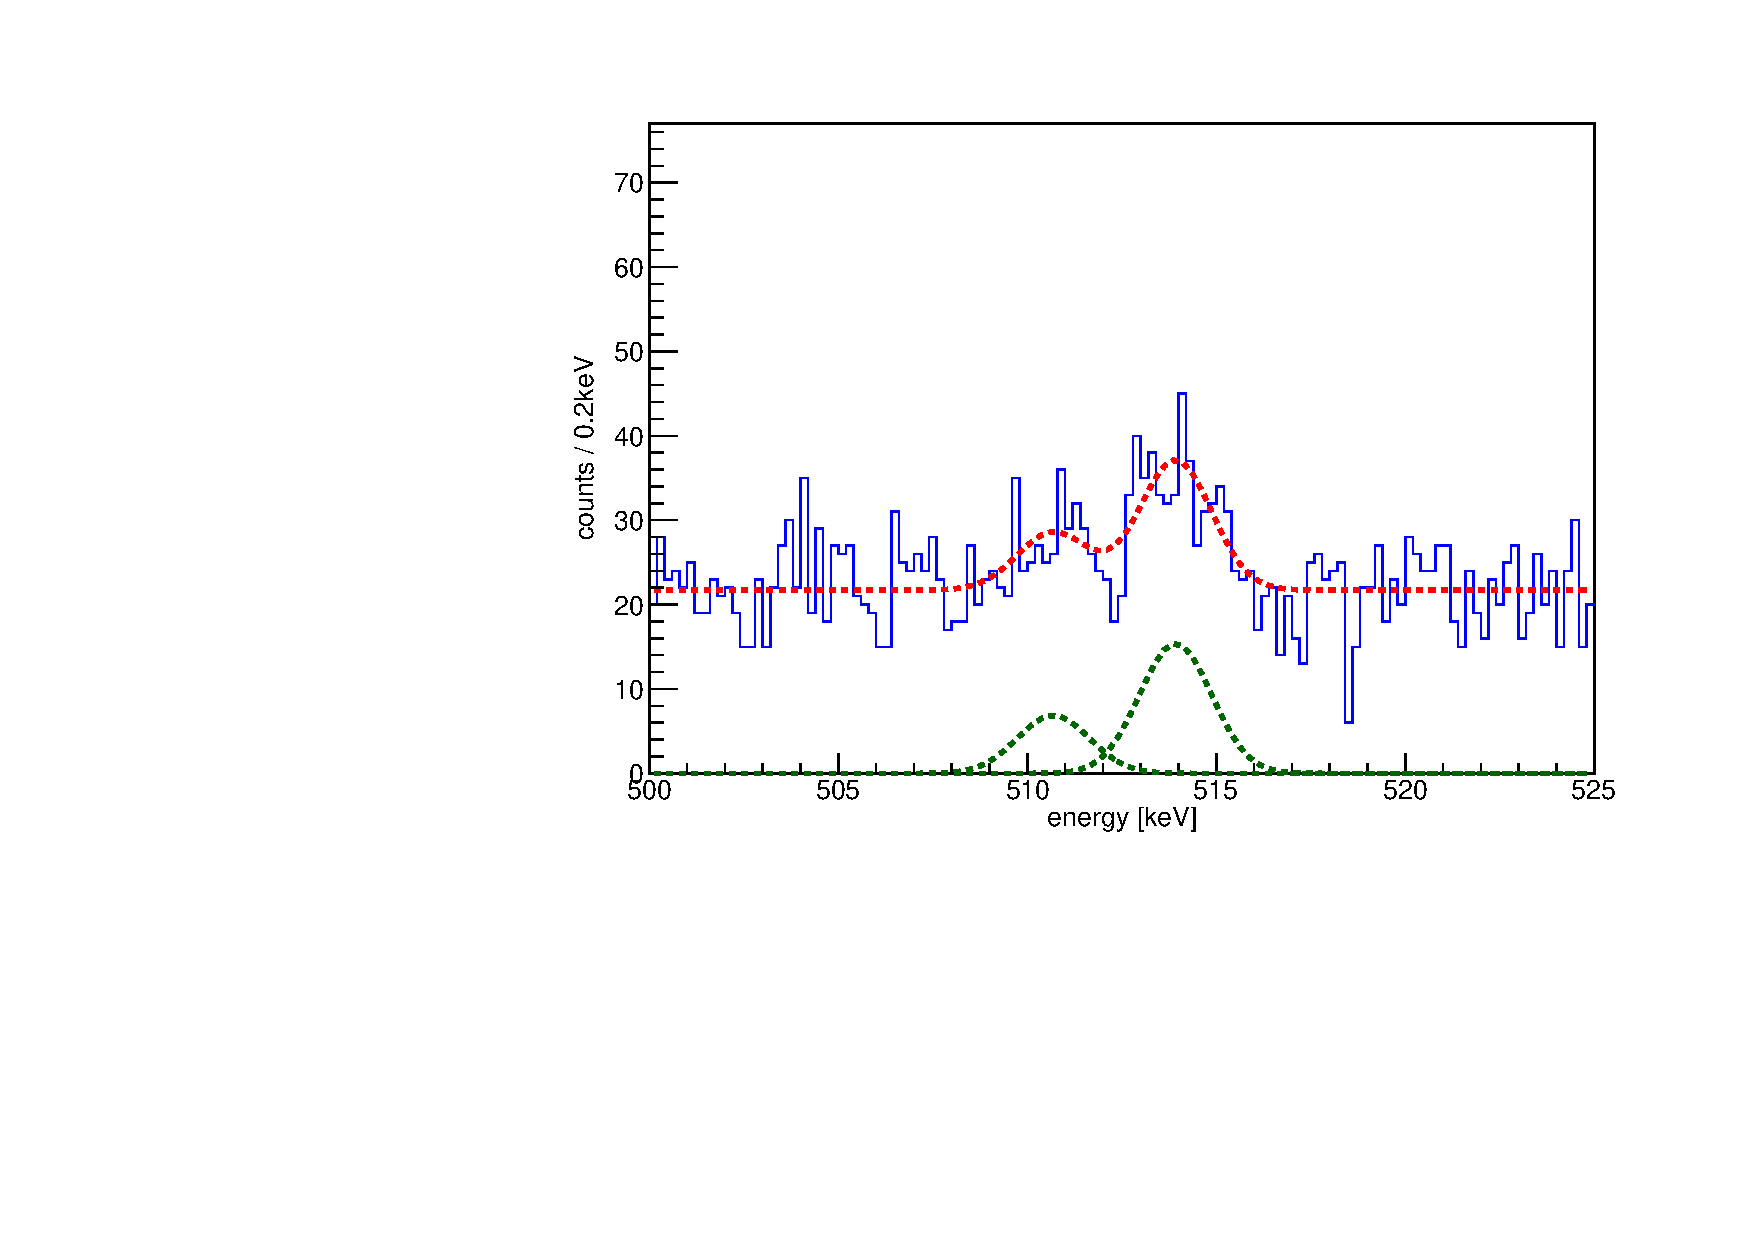
\includegraphics[width=80mm]{./Bilder/500525FitNoFilterBEGes.pdf}
		\caption{BEGes}
		\label{fig:FitNoFilterBEGes}
	\end{minipage}%
	\begin{minipage}{.5\textwidth}
		\centering
		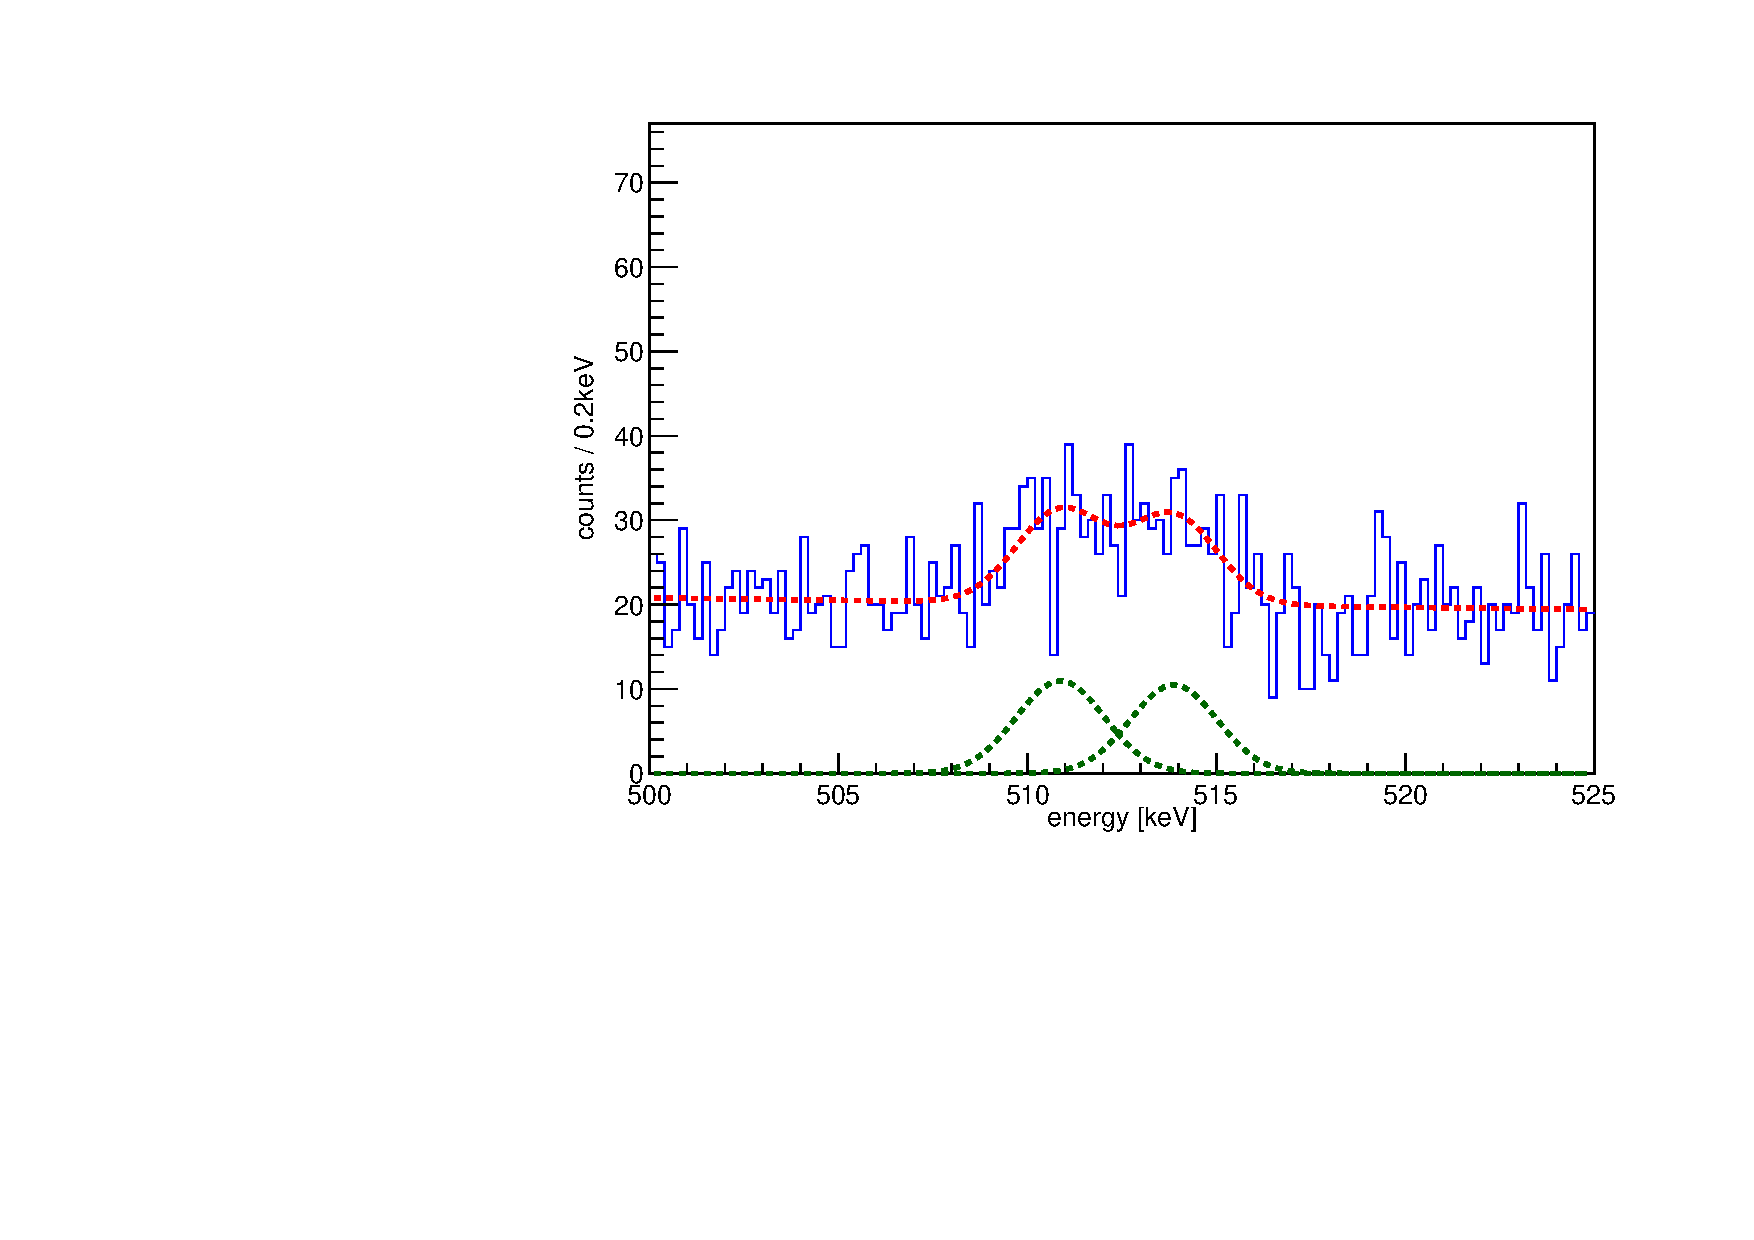
\includegraphics[width=80mm]{./Bilder/500525FitNoFilterCOAX.pdf}
		\caption{COAX}
		\label{fig:FitNoFilterCOAX}
	\end{minipage}
    \\
	\vspace{0.5cm}
	All events measured by the respective detectors in the range of 500keV to 525keV fitted with a fit function in the form seen in equation \ref{equ:FitNoFilters}. The green function represent the two Gaussian peaks independently using the determined fit parameters.
\vspace{0.5cm}
\end{figure}
\\

\begin{figure}[t!]
\centering
\begin{tabular}{|c|c|c}
\hline
Name	& Value [BEGes] & Valuse [COAX]\\ 
\hline
A  &	(16.15 \(\pm\)	3.658)&	(29.842 \(\pm\)	3.968)	\\	
\hline
B  &	(510.693 \(\pm\)	0.564)&	(510.750 \(\pm\)	0.265)\\	
\hline
C  &	(1.022 \(\pm\)	1.433)	&	(1.564 \(\pm\)	0.236	)	\\
\hline
D  &	(27.239 \(\pm\)	3.870)	&	(20.463 \(\pm\)	3.279	)	\\
\hline
E  &	(513.940 \(\pm\)	0.701)	&	(513.858 \(\pm\)	0.213)	\\
\hline
F  &	(0.909 \(\pm\)	1.400)	&	(1.017 \(\pm\)	0.173	)	\\
\hline
G  &	(14.175 \(\pm\)	1.050)	&	(13.123 \(\pm\)	0.289	)	\\
\hline
H  &	(24.487 \(\pm\)	1.833)	&	(-384995.062 \(\pm\)	2.592)	\\
\hline
I  &	(-40.573 \(\pm\) 1.000)	&	(-40.573 \(\pm\)	1.414)\\
\hline

\end{tabular}
\label{tab:FitParNoFilter}
\captionof{table}[]{Fit parameters of fit function \ref{equ:FitNoFilters} applied on the phase-space diagram of the respective detectors.}
\end{figure}
\\

The only values of these fit parameters that is of real interest for the determination of the activity is variable D.
Its value is the amplitude of the second Gaussian peak.
Because the Gaussian peak was chosen in the normalized form this value also represents the amount of rare \nuc{Kr}{85} decays measured.
This means that from the hardly filtered events over the entire course of phase II an amount of (27.24\(\pm\)3.88) rare \nuc{Kr}{85} decays were measured in the BEGe detectors and (20.46\(\pm\)3.28) in the COAX detectors. 
\\

Now to the two liquid argon filtered cases.
Before we apply the fits we have to discus what we are expecting.
In the ideal case, that the majority of all rare \nuc{85}{85} decays through the liquid argon filter, we expect the amplitude of the Gaussian peaks in both the LArVeto filtered case and the hardly filtered case to be similar.
These results would then be used in the further course of the analysis, since their values gather more directly than the results of the hardly filtered case.
In contrast, in the case that a not insignificant amount of \nuc{Kr}{85} decays was filtered out that this amplitude is expected to be much smaller.
If this were to happen, we would have to fall back on the results of the hardly filtered values.
\\

Now to actually applying the fits.
As mentioned above we can assumed that the positron electron annihilation peak is fully suppressed.
Therefor only one Gaussian peak has to be fitted together with the background function.
The fit therefor results in the function displayed in equation \ref{equ:FitFilters}.
\\ 

\begin{equation}
\mathrm{f}(x) = \mathrm{A}\frac{1}{\sqrt{2\pi\mathrm{C}}}\exp\left(-\frac{(x-\mathrm{B})^2}{2\mathrm{C}^2}\right) + \mathrm{D}\exp\left(\mathrm{E}x\right) + \mathrm{F}
\label{equ:FitFilters}
\end{equation}

After applying the fit to the four phase-space diagrams seen in figure \ref to \ref, you get the fit parameters displayed in table

\begin{figure}[t!]
	\centering
	\begin{minipage}{.5\textwidth}
		\centering
		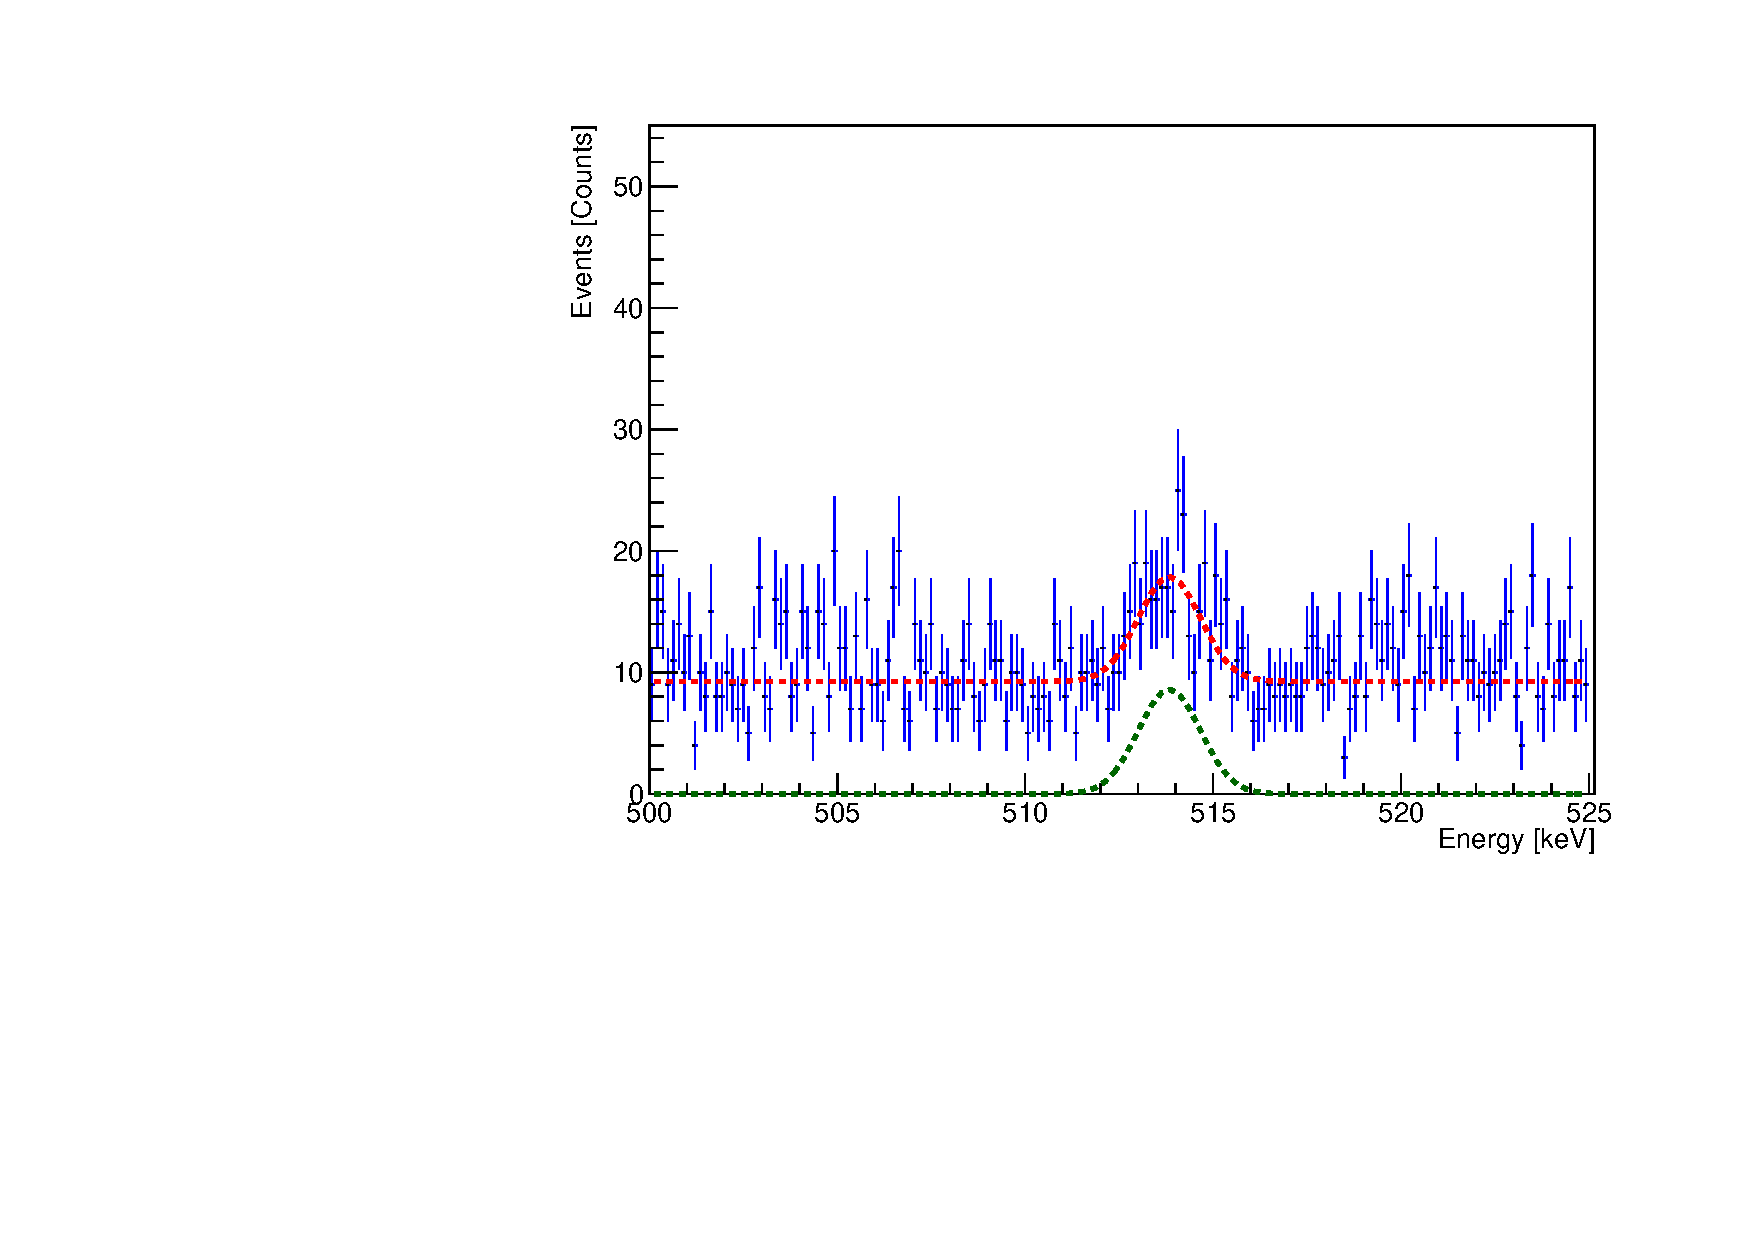
\includegraphics[width=80mm]{./Bilder/500525FitLArVetoBEGes.pdf}
		\caption{BEGes}
		\label{fig:FitLArVetoBEGes}
	\end{minipage}%
	\begin{minipage}{.5\textwidth}
		\centering
		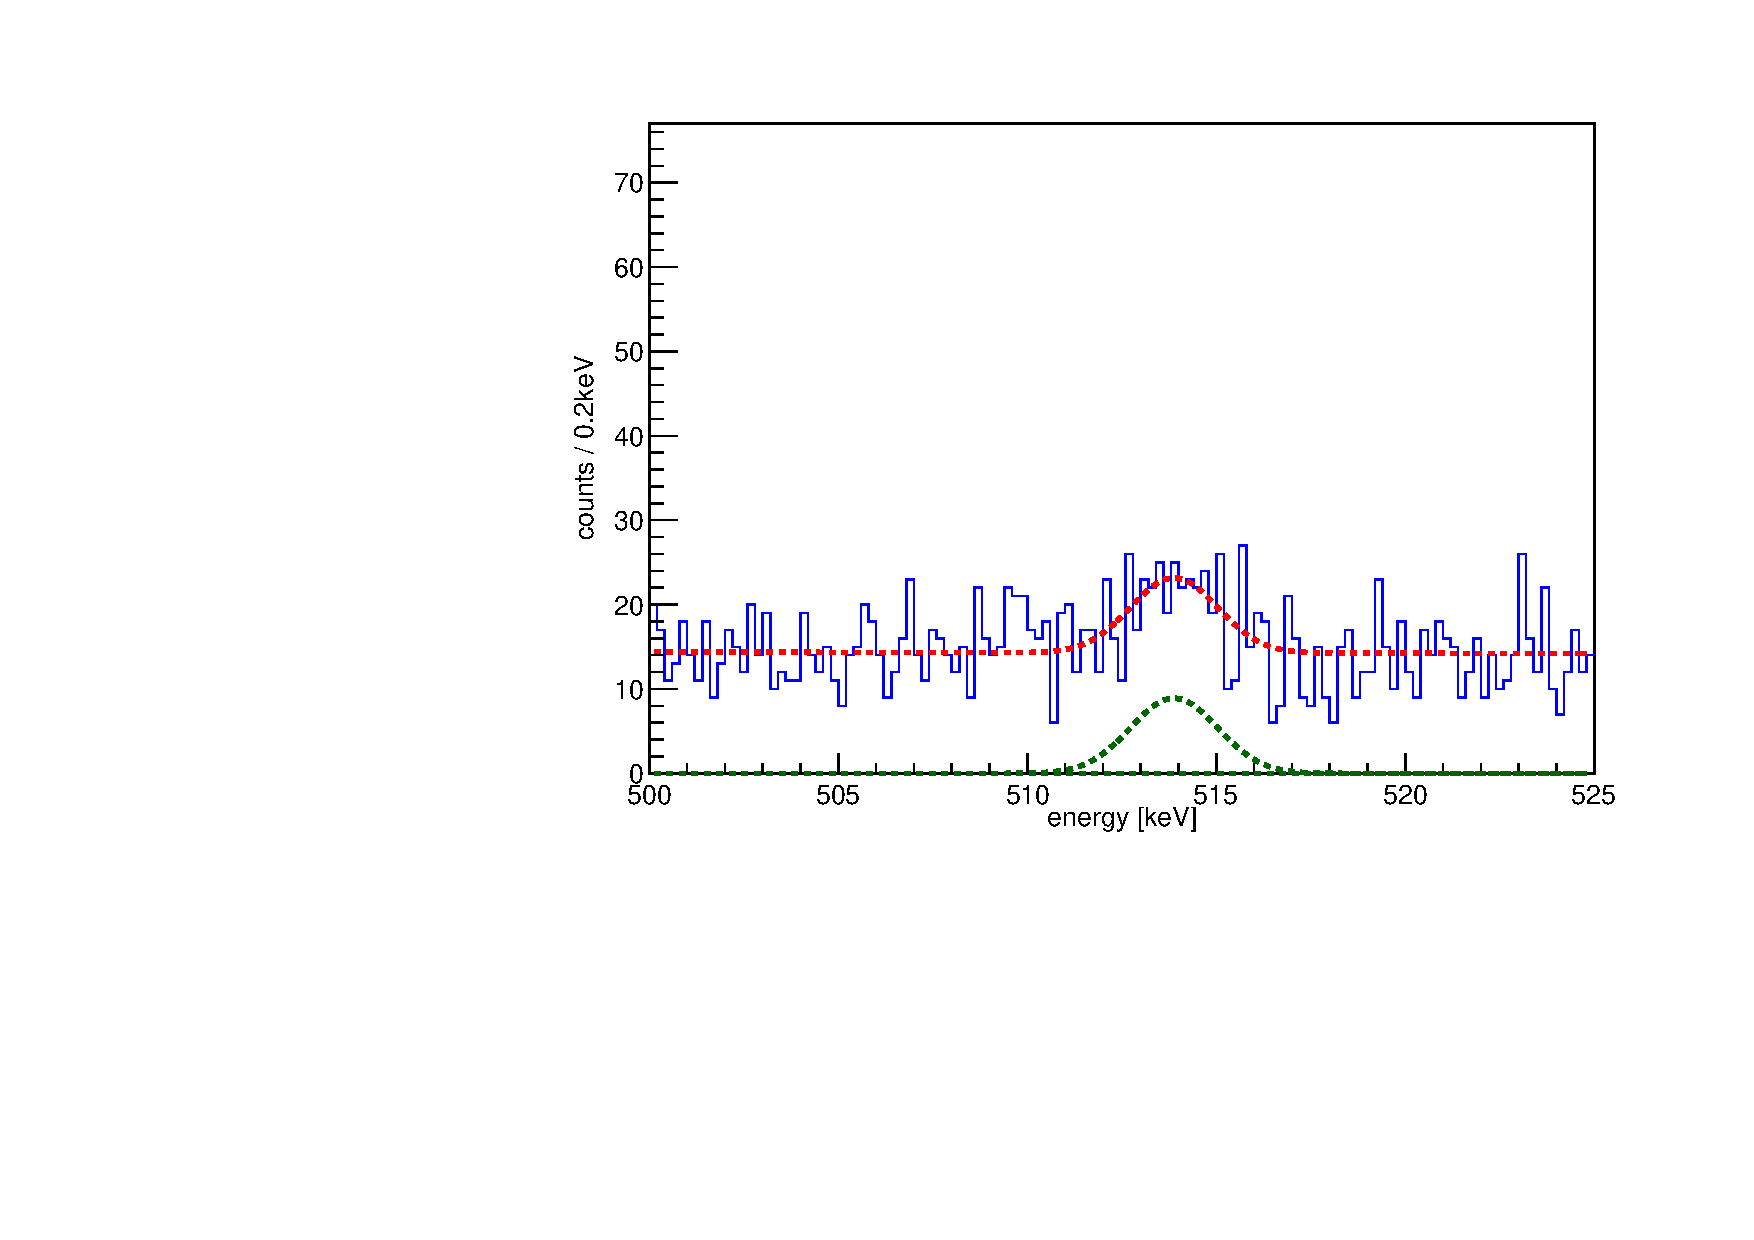
\includegraphics[width=80mm]{./Bilder/500525FitLArVetoCOAX.pdf}
		\caption{COAX}
		\label{fig:FitLArVetoCOAX}
	\end{minipage}
	\\
	\vspace{0.5cm}
	All events measured by the respective detectors  with the liquid argon veto applied in the range of 500keV to 525keV fitted with a fit function in the form seen in equation \ref{equ:FitFilters}.
	\\
	\vspace{0.5cm}
	\begin{minipage}{.5\textwidth}
		\centering
		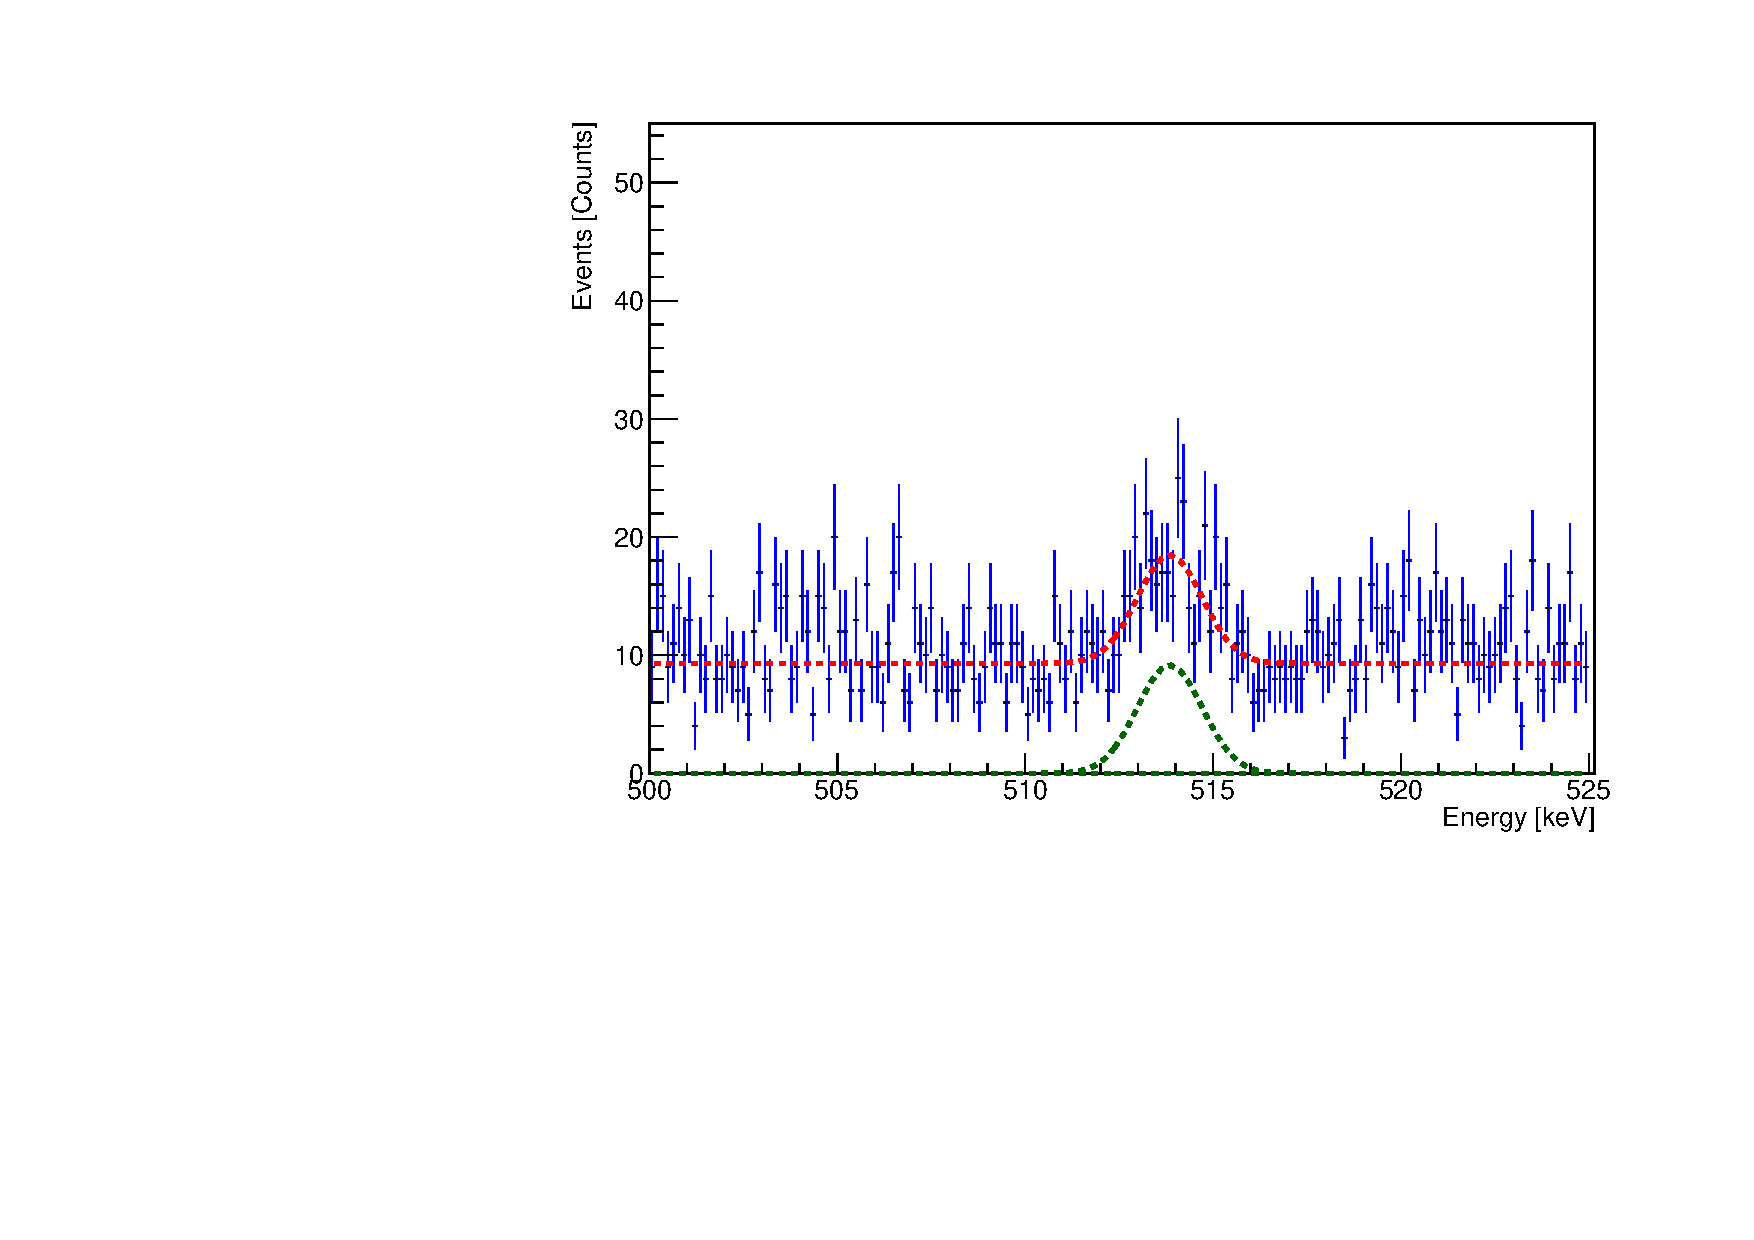
\includegraphics[width=80mm]{./Bilder/500525FitLArVetoEventListBEGes.pdf}
		\caption{BEGes}
		\label{fig:FitLArVetoEventListBEGes}
	\end{minipage}%
	\begin{minipage}{.5\textwidth}
		\centering
		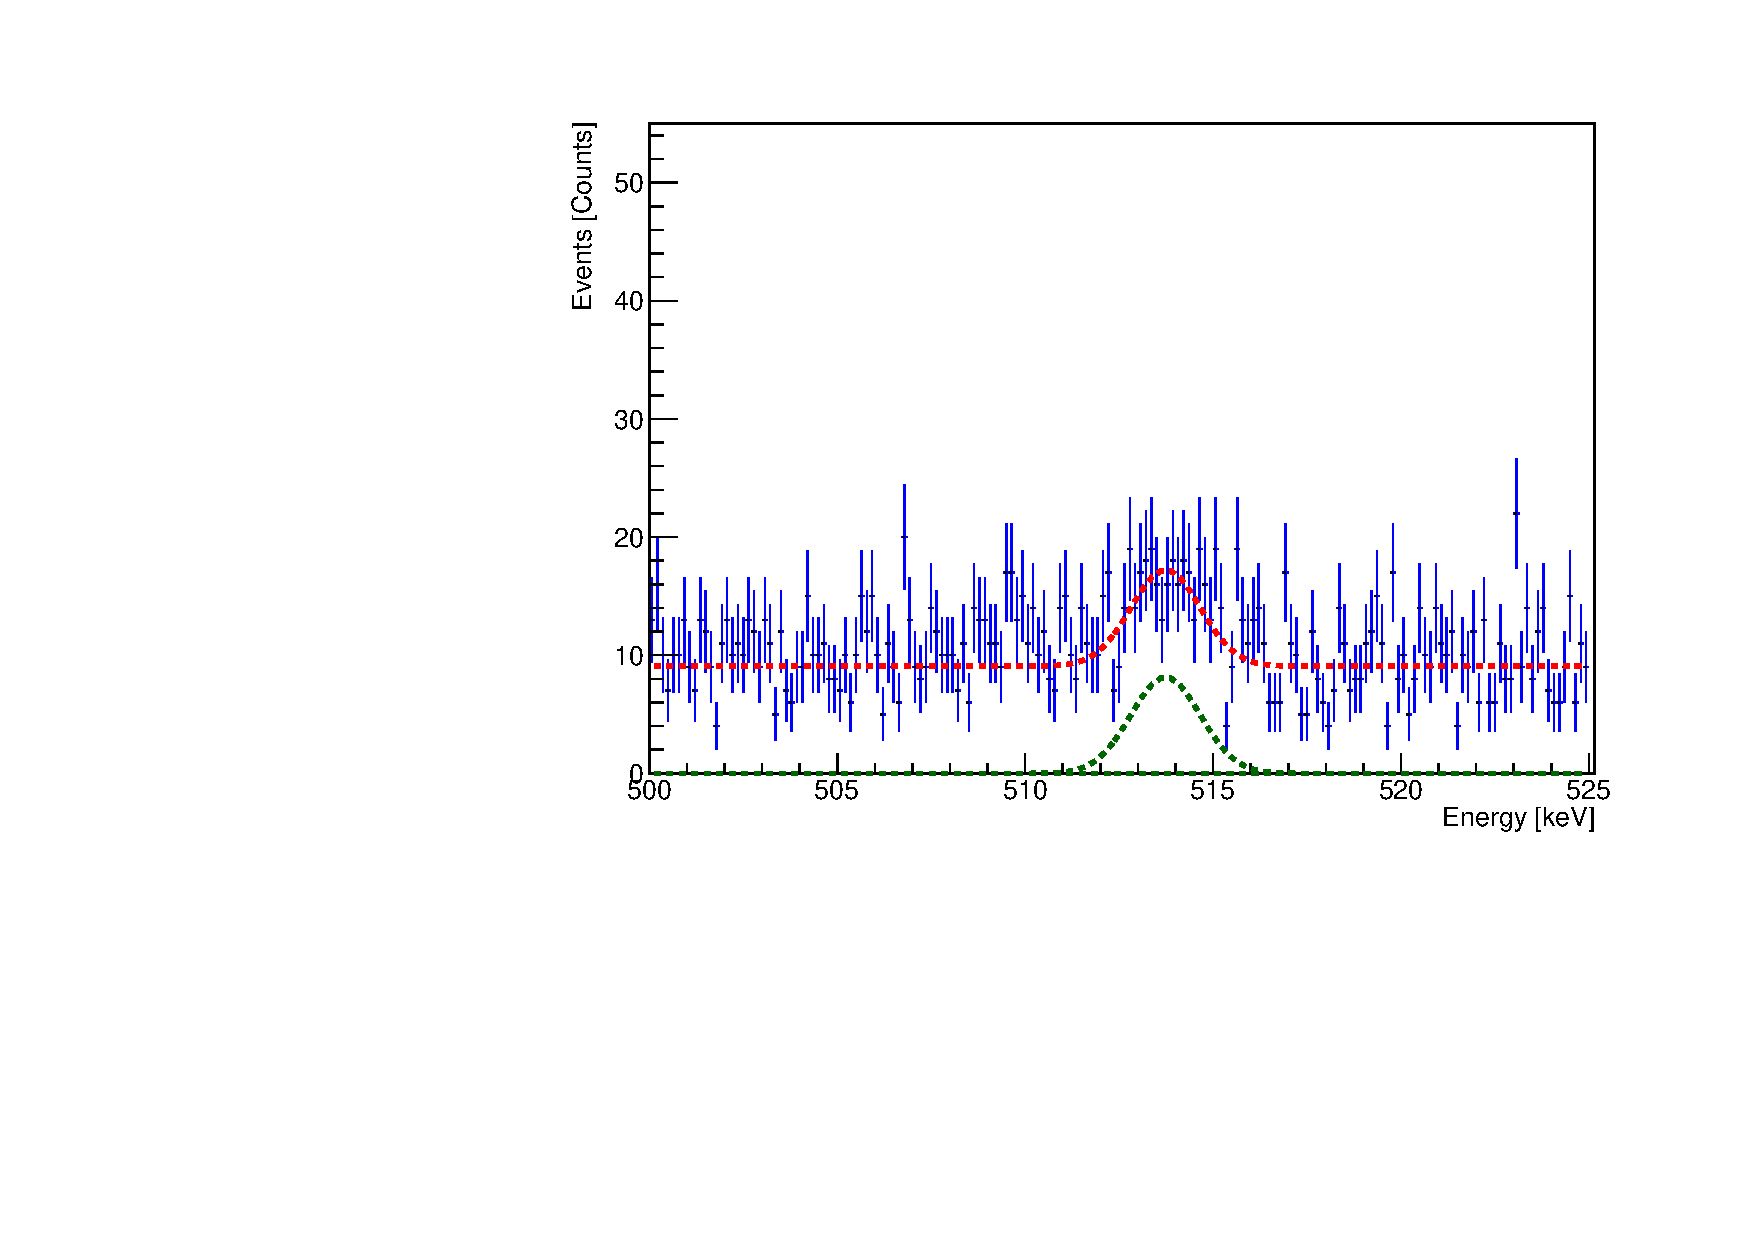
\includegraphics[width=80mm]{./Bilder/500525FitLArVetoEventListCOAX.pdf}
		\caption{COAX}
		\label{fig:FitLArVetoEventListCOAX}
	\end{minipage}
	\\
	\vspace{0.5cm}
	All events measured by the respective detectors with the liquid argon veto applied and the falsely filtered \nuc{Kr}{85} events recovered in the range of 500keV to 525keV fitted with a fit function in the form seen in equation \ref{equ:FitFilters}.
	!!!!! god dammit da muss man zwei vlt drei sätze draus machen!!!!!
	\vspace{0.5cm}
\end{figure}
\\

\begin{figure}[t!]
	\centering
	\begin{tabular}{|l|r|r|r|r|}
		\hline
		Name	& Value [BEGes] \\ 
		\hline
		A  &	(17.844639 \(\pm\)	3.179471)&	(17.914476 \(\pm\)	2.683260)	&	(19.847330\(\pm\)	2.688415)&	(18.851511 \(\pm\)	2.696000)\\	
		\hline
		B  &	(513.838989 \(\pm\)	0.665171)&	(513.748535 \(\pm\)	0.179167)&	(513.849854 \(\pm\)	0.152052)&	(513.737183	\(\pm\) 0.167941)\\	
		\hline
		C  &	(0.828315 \(\pm\)	1.377836)	&	(0.940856 \(\pm\)	0.160788	)	&	(0.865958\(\pm\) 0.108436)&	(0.923679 \(\pm\)	0.149867)\\
		\hline
		D  &	(9.265341 \(\pm\)	1.032088)	&	(9.073170 \(\pm\)	0.233725	)	&	(9.307535\(\pm\)	0.236841)&	(9.076473 \(\pm\)	0.233940)\\
		\hline
		E  &	(18.142975 \(\pm\)	1.833031)	&	(-401772.843750 \(\pm\)	3.666062)	&	(-394189.968750\(\pm\)	45.660984)&	(-796827.062500 \(\pm\)	64.574379)\\
		\hline	
		F  &	(-26.647284 \(\pm\)	1.000000)	&	(-43.877174 \(\pm\)	1.414214	)	&	(-55.546192\(\pm\)	1.414214)&	(-55.546192 \(\pm\)	1.414214)\\
		\hline
	\end{tabular}
	\label{tab:FitParNoFilter}
	\captionof{table}[]{Fit parameters of fit function \ref{equ:FitNoFilters} applied on the phase-space diagram of the respective detectors.}
\end{figure}
\\


As above, the amplitude A of the Gaussian peak correspond to the number of events measured by this peak.
In the case of only applying the liquid argon veto it can be seen that the number of events in the BEGe and in the COAX detectors has dropped considerably compared to the hardly filtered value.
This shows that a recovery of falsely filtered rare \nuc{Kr}{85} decays is necessary.
But even in these cases, the amplitudes of the peaks is still much smaller, at least in the case of the BEGes.
\\



% calculate Amplitude of Gauss peak at 514keV and use factor from Monte Carlo Simulation to estimate

% look at phase diagram at range of 500 to 525 keV, use different filters and fit remaining data with Gaussian function
% -> get amplitude
% make a Monte Carlo simulation to estimate actual Kr85 activity in LAr from measured activity in detectors
% -> with amplitude and factors from MC-Simulation one can calculate the specific activity

\subsection{Activity from the decrease in rate}
\label{sec:SAfromDecrease}

% use fit to calculate the decrease in rate of the signals in range from 200 to 500keV
% from fit and assumption that only Kr85's activity is decreasing one can calculate the specific activity from the amplitude of the fit

% use Volume of LAr-Tank to determine the number of Kr85 and from this the concentration in the argon

\subsection{Calculation of the concentration}
\label{sec:calcOfTheCon}


\section{Conclusion}

% what went wrong?
% what does it mean?
% possible future enhancements to determine the Kr85 concentration

































% %%%%%%%%%%%%%%%%%%%%%%%%%%%%%%%%%%%%%%%%%%%%%%%%%%%%%%%%%%%%%%%%%%%%%%%%%%%%%%%%
% \section{Another Section}
% \label{sec:secname}


% Fig.~\ref{fig:pmt} shows a PMT.

% %------------------------------------------------------------------- figure ----
% \begin{figure}[hb]
% \centering
% \ifmakefigures%
%    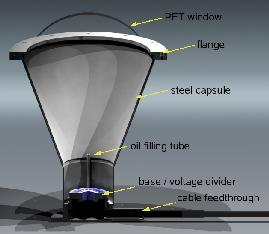
\includegraphics[width=45mm]{kapselung-small.jpg}
% \fi%
%   \caption{\label{fig:pmt}
% The encapsulation of the Cerenkov PMT.
% }
% \end{figure}
% %-------------------------------------------------------------------------------

% %%%%%%%%%%%%%%%%%%%%%%%%%%%%%%%%%%%%%%%%%%%%%%%%%%%%%%%%%%%%%%%%%%%%%%%%%%%%%%%%
% \section{Results and Analysis}
% \label{sec:results}


% %----------------------------------------------------------------- equation ----
% {\centering
% \begin{equation}\label{eq:sensit}
%     T_{1/2}(0^{+} \rightarrow g.s.~with~single~\gamma)~ \geq ~\ln2 \cdot
%     \varepsilon \cdot a \cdot \frac{M \cdot N_A}{A} \cdot 
%     \sqrt{\frac{\Delta T}{b\cdot\Delta E}},
% \end{equation}
% } % end centering
% %-------------------------------------------------------------------------------

% Table~\ref{tab:param} compiles everything.

% %-------------------------------------------------------------------- table ----
% \begin{table}[t]
% \centering
% \caption{\label{tab:param}
% Experimental parameters and values.
% }
% \vspace*{2mm}
% \begin{tabular}{L{4cm}|C{6cm}}
%   Column1 & Column2 \\  \hline 
%   Row1 & $100\pm10$ \\
%   Row2 & $100\pm10$ \\ \hline
%   Row3 & $100\pm10$ \\
%   Row4 & $100\pm10$ \\ 
% \end{tabular}
% \end{table}
% %-------------------------------------------------------------------------------

% %%%%%%%%%%%%%%%%%%%%%%%%%%%%%%%%%%%%%%%%%%%%%%%%%%%%%%%%%%%%%%%%%%%%%%%%%%%%%%%%
% \section{Conclusions}
% \label{sec:conclusions}
